% arara: makeindex

% Template for IEEE papers
%% bare_conf.tex
%% V1.4b
%% 2015/08/26
%% by Michael Shell
%% See:
%% http://www.michaelshell.org/
%% for current contact information.
%%
%% This is a skeleton file demonstrating the use of IEEEtran.cls
%% (requires IEEEtran.cls version 1.8b or later) with an IEEE
%% conference paper.
%%
%% Support sites:
%% http://www.michaelshell.org/tex/ieeetran/
%% http://www.ctan.org/pkg/ieeetran
%% and
%% http://www.ieee.org/

%%*************************************************************************
%% Legal Notice:
%% This code is offered as-is without any warranty either expressed or
%% implied; without even the implied warranty of MERCHANTABILITY or
%% FITNESS FOR A PARTICULAR PURPOSE!
%% User assumes all risk.
%% In no event shall the IEEE or any contributor to this code be liable for
%% any damages or losses, including, but not limited to, incidental,
%% consequential, or any other damages, resulting from the use or misuse
%% of any information contained here.
%%
%% All comments are the opinions of their respective authors and are not
%% necessarily endorsed by the IEEE.
%%
%% This work is distributed under the LaTeX Project Public License (LPPL)
%% ( http://www.latex-project.org/ ) version 1.3, and may be freely used,
%% distributed and modified. A copy of the LPPL, version 1.3, is included
%% in the base LaTeX documentation of all distributions of LaTeX released
%% 2003/12/01 or later.
%% Retain all contribution notices and credits.
%% ** Modified files should be clearly indicated as such, including  **
%% ** renaming them and changing author support contact information. **
%%*************************************************************************


% *** Authors should verify (and, if needed, correct) their LaTeX system  ***
% *** with the testflow diagnostic prior to trusting their LaTeX platform ***
% *** with production work. The IEEE's font choices and paper sizes can   ***
% *** trigger bugs that do not appear when using other class files.       ***                          ***
% The testflow support page is at:
% http://www.michaelshell.org/tex/testflow/

\documentclass{book}
\usepackage[quiet]{fontspec}
\usepackage[table,xcdraw,dvipsnames]{xcolor} % Used by spritegrid and others.
\usepackage[obeyspaces,spaces]{url}
\usepackage{longtable}
\usepackage{arydshln}
\usepackage{booktabs}
\usepackage{afterpage}
\usepackage{flushend}
\usepackage{titletoc}
\usepackage[toc]{appendix}
\usepackage{parskip}
\usepackage{graphicx,wrapfig}
\usepackage{float}
\usepackage{caption}
\usepackage{pdfpages}
\usepackage{tikzpagenodes}
\usepackage{imakeidx}
\usepackage[pagestyles,raggedright]{titlesec}
\usepackage[all]{nowidow}
\usepackage[bookmarks=true,linktoc=all]{hyperref}
\hypersetup{
  colorlinks   = true, %Colours links instead of ugly boxes
  urlcolor     = blue, %Colour for external hyperlinks
  % Each main .tex file configures via \titleformat the \chapter command
  % to do {\chapmtoc\insertminitoc} and \chapmtoc, as defined below, will
  % use \hypersetup{linkcolor=white} to avoid blue-on-blue TOC links
  % Besides, each main .tex file will issue the \tableofcontents command
  % between \hypersetup{linkcolor=black} and \hypersetup{linkcolor=blue}
  % This means however that if "blue" is modified here it must be modified
  % in these files too.
  linkcolor    = blue, %Colour of internal links
  citecolor   = red %Colour of citations
}
\usepackage{aeb-minitoc}
\usepackage{fix-cm}
\usepackage{textpos}
\usepackage{enumitem}
\usepackage{tcolorbox}
\tcbuselibrary{breakable,listings,skins,xparse}
%\usepackage{wrapfig}
\usepackage{needspace}
\usepackage{verbatim}
\usepackage{ean13isbn}
\usepackage{setspace}

% Use CHAPTER-PAGE page numbering to make it easier to modify chapters
% later, without messing up page number of the rest of the book.
\usepackage[auto]{chappg}

% Allow cross-references between the various books to the big The MEGA65 Book
\usepackage{xr}
\usepackage{varioref}
\usepackage{xparse}
\externaldocument[M65Book-]{mega65-book}
% And a \ref alternative that checks if it needs to be a cross-reference to the
% MEGA65 Book instead.
\makeatletter
\newcommand{\bookref}[1]{%
    \@ifundefined{r@#1}{%
      {\em the MEGA65 Book}, \nameref{M65Book-#1} (\autoref{M65Book-#1})}{\autoref{#1}}%
}
\newcommand{\bookvref}[1]{%
    \@ifundefined{r@#1}{%
      {\em the MEGA65 Book}, \nameref{M65Book-#1} (\autoref{M65Book-#1})}{Chapter/Appendix \vref{#1}}%
}
\makeatother

% For fixed-width columns in register maps
\usepackage{array}

% Makes tables with double-ruled lines look better
\usepackage{hhline}

% Makes better use of space for reference tables in appendix
\usepackage{multicol}

% Shaded tables with alternate rows colored for better legibility
% Best used with larger tables rather than small tables
\usepackage{colortbl}
\usepackage{adjustbox}
\usepackage[strict]{changepage}

% \makecell command for forcing line breaks in table cells
\usepackage{makecell}

\newcolumntype{L}[1]{>{\raggedright\let\newline\\\arraybackslash\hspace{0pt}}m{#1}}
\newcolumntype{C}[1]{>{\centering\let\newline\\\arraybackslash\hspace{0pt}}m{#1}}
\newcolumntype{R}[1]{>{\raggedleft\let\newline\\\arraybackslash\hspace{0pt}}m{#1}}

% clear to left page for making two page tables starting on the odd page
\newcommand{\cleartoleftpage}{%
  \clearpage
  \ifodd\value{page}\hbox{}\newpage\fi
}

% For displaying Letter keys and the MEGA key
% This is a `keys' element for displaying a Mega65 keyboard key
% using a black filled label with rounded edges.
% In order to display a key as a title, use:
%
%     \megakey[title]{Run/Stop}
%
% For displaying a key as a part of the normal document flow, simply use:
%
%    \specialkey{SHIFT}
%
%
% If you get warnings on special characters, mathematical characters etc, use $, eg:
%
%    \megakey{$\leftarrow$}
%
% Other sizes are supported, as part of tcolorbox:
% http://mirror.aarnet.edu.au/pub/CTAN/macros/latex/contrib/tcolorbox/tcolorbox.pdf#subsubsection.4.7.5 however, only `title' and the default: `small' are proposed for use in this manual.
%
% The second macro available here is the megasymbolkey.
% This will display the MEGA symbol as white on a black key box. Simply use:
%
%		 \megasymbolkey
%
% Some MEGA65 keys contain two lines of text like "RUN/STOP"
% You can use the specialkey macro for this:
%
%    \specialkey{SHIFT LOCK}%

\usepackage{tcolorbox}

\newtcbox{\megakeyinner}[1][small]{colback=black, coltext=white, size=#1, fontupper=\bfseries, nobeforeafter,box align=bottom,baseline=3pt,text height=7pt,valign=center}
\newcommand{\megakey}[2][small]{\megakeyinner[#1]{\uppercase{#2}}}

\newtcbox{\megakeyinnerwhite}[1][small]{colback=white, coltext=black, size=#1, fontupper=\bfseries, nobeforeafter,box align=bottom,baseline=3pt,text height=7pt,valign=center}
\newcommand{\megakeywhite}[2][small]{\megakeyinnerwhite[#1]{\uppercase{#2}}}

% Previous version of megasymbolkey
%\newtcbox{\megasymbolkeyinner}{colback=black, coltext=white, clip title=false. fontupper=\symbolfont, box align=bottom,baseline=3pt,text height=7pt}
%\newcommand{\megasymbolkey}{\megakeyinner{\megasymbol[white]}\ }

\newtcolorbox{megasymbolkeyinner}
{colback=black,coltext=white,size=small,fontupper=\small\bfseries,
width=0.65cm, height=0.55cm, box align=base,
nobeforeafter, halign=flush left, left=0mm,top=0.3mm,bottom=0mm,right=0mm
,boxsep=0.5mm,baseline=4pt, enlarge right by = 1mm
}
\newcommand{\megasymbolkey}{
\begin{megasymbolkeyinner}%
\megasymbol[white]%
\end{megasymbolkeyinner}%
}

\newtcolorbox{specialkeyinner}
{colback=black,coltext=white,size=small,fontupper=\tiny\bfseries,
width=0.80cm, height=0.55cm, box align=base,
nobeforeafter, halign=flush left, left=0mm,top=0.3mm,bottom=0mm,right=0mm
,boxsep=0.5mm,baseline=4pt
}
\newcommand{\specialkey}[1]{
\begin{specialkeyinner}%
#1%
\end{specialkeyinner}%
}

\newtcolorbox{widekeyinner}
{colback=black,coltext=white,size=small,fontupper=\tiny\bfseries,
width=0.9cm, height=0.55cm, box align=base,
nobeforeafter, halign=flush left, left=0mm,top=0.3mm,bottom=0mm,right=0mm
,boxsep=0.5mm,baseline=4pt
}
\newcommand{\widekey}[1]{
\begin{widekeyinner}%
#1%
\end{widekeyinner}%
}




% For displaying print versions petscii character symbols
\input{elements/graphicsymbol}

% For Mega65 display of code, listings and screen activity
% This is a collection of elements for displaying output from the Mega65 screen.
% They can display program code or fragments to show activity on the screen.
% Example of use:
%
%    \begin{screencode}
%    10 OPEN 1,8,0,"$0:*,P,R
%    20 : IF DS THEN PRINT DS$: GOTO 100
%    30 GET#1,X$,X$
%    40 DO
%    50 : GET#1,X$,X$: IF ST THEN EXIT
%    60 : GET#1,BL$,BH$
%    70 : LINE INPUT#1, F$
%    80 : PRINT LEFT$(F$,18)
%    90 LOOP
%    100 CLOSE 1
%
%    RUN
%    \end{screencode}
%
% for inline display of code, use:
%
%    \screentext{?SYNTAX ERROR}
%

\usepackage{listings,color}

\lstnewenvironment{screenoutputlined}
   {
     \lstset{
               basicstyle=\codefont\color{white}\linespread{1.0}\normalsize,
               backgroundcolor=\color{black},fillcolor=\color{black},
               rulecolor=\color{black},
               frame=lines,
               framexleftmargin=2mm,
               framexrightmargin=2mm,
               framextopmargin=2mm,
               framexbottommargin=2mm,
               tabsize=4,
               xleftmargin=2mm,
               xrightmargin=2mm,
               basewidth={0.4em},
               literate={\*}{*}1{\-}{-}1{\/}{/}1{{\ }}{{ }}1
            }
   }
   {  }

\lstdefinestyle{megalisting}{basicstyle=\codefont\normalsize,breaklines=false,fontadjust=true,basewidth=1.5mm}
\makeatletter
\newtcblisting{screencode}{%
listing only,
colback=black,
coltext=white,
boxsep=0mm,
left=2mm,
right=0mm,
top=-1mm,
bottom=-1mm,
listing options={style=megalisting},
% Gets ignored by listings package
%fontupper=,
%enlarge left by =\csname @totalleftmargin\endcsname
}
\makeatother

% Stop - signs in listings getting turned into minus characters
\makeatletter
\lst@CCPutMacro
    \lst@ProcessOther {"2D}{\lst@ttfamily{-{}}{-}}
    \@empty\z@\@empty
% Also stop * being pushed down or faultily verically centred
\lst@CCPutMacro
    \lst@ProcessOther {"2A}{%
      \lst@ttfamily
         {{*}}% used with ttfamily
         {*}}% used with other fonts
    \@empty\z@\@empty
\makeatother


% For in-line screen text
\newcommand{\screentext}[1]{{\codefont\color{black}\normalsize{#1}}}
\newcommand{\screentextwide}[1]{{\codefontwide\color{black}\small{#1}}}
% Just to save typing
\newcommand{\stw}[1]{{\codefontwide\color{black}\small{#1}}}

% 45GS02 assembler mneomics and Acme directives
\lstdefinelanguage[45gs02]{Assembler}%
  {morekeywords={%
    adc,and,asl,asr,asw,aug,bbr0,bbr1,bbr2,%
    bbr3,bbr4,bbr5,bbr6,bbr7,bbs0,bbs1,bbs2,%
    bbs3,bbs4,bbs5,bbs6,bbs7,bcc,bcs,beq,%
    bit,bmi,bne,bpl,bra,brk,bsr,bvc,%
    bvs,clc,cld,cle,cli,clv,cmp,cpx,%
    cpy,cpz,dec,dew,dex,dey,dez,eom,%
    eor,inc,inw,inx,iny,inz,jmp,jsr,%
    lda,ldx,ldy,ldz,lsr,map,neg,nop,%
    ora,pha,php,phw,phx,phy,phz,pla,%
    plp,plx,ply,plz,rmb0,rmb1,rmb2,rmb3,%
    rmb4,rmb5,rmb6,rmb7,rol,ror,row,rti,%
    rts,sbc,sec,sed,see,sei,smb0,smb1,%
    smb2,smb3,smb4,smb5,smb6,smb7,sta,stx,%
    sty,stz,tab,tax,tay,taz,tba,trb,%
    tsb,tsx,tsy,txa,txs,tya,tys,tza,%
    adcq,andq,aslq,asrq,bitq,cmpq,deq,eorq,%
    inq,ldq,lsrq,orq,rolq,rorq,sbcq,stq},%
  morekeywords=[2]{%
    !8,!08,!by,!byte,!16,!wo,!word,!le16,%
    !be16,!24,!le24,!be24,!32,!le32,!be32,!hex,%
    !h,!fill,!fi,!skip,!align,!convtab,!ct,!text,%
    !tx,!pet,!raw,!scr,!scrxor,!to,!source,!src,%
    !binary,!bin,!zone,!zn,!symbollist,!sl,!if,!ifdef,%
    !ifndef,!for,!set,!do,!while,!endoffile,!eof,!warn,%
    !error,!serious,!macro,!initmem,!xor,!pseudopc,!cpu,!al,!as,!rl,!rs,!address,!addr,
  },%
  alsoletter=.,%
  alsodigit=?,%
  sensitive=f,%
  morestring=[b]",%
  morestring=[b]',%
  morecomment=[l]{;}%
  }[keywords,comments,strings]

\lstdefinelanguage[MEGA65]{Basic}%
  {morekeywords={%
    end,for,next,data,input\#,input,dim,read,%
    let,goto,run,if,restore,gosub,return,rem,%
    stop,on,wait,load,save,verify,def,poke,%
    print\#,print,cont,list,clr,cmd,sys,open,%
    close,get,new,tab,to,fn,spc,then,%
    not,step,+,-,*,/,\^,and,%
    or,>,=,<,sgn,int,abs,usr,%
    fre,pos,sqr,rnd,log,exp,cos,sin,%
    tan,atn,peek,len,str\$,val,asc,chr\$,%
    left\$,right\$,mid\$,go,rgraphic,rcolor,joy,rpen,%
    dec,hex\$,err\$,instr,else,resume,trap,tron,%
    troff,sound,vol,auto,import,graphic,paint,char,%
    box,circle,paste,cut,line,merge,color,scnclr,%
    xor,help,do,loop,exit,dir,dsave,dload,%
    header,scratch,collect,copy,rename,backup,delete,renumber,%
    key,monitor,using,until,while,bank,filter,play,%
    tempo,movspr,sprite,sprcolor,rreg,envelope,sleep,catalog,%
    dopen,append,dclose,bsave,bload,record,concat,dverify,%
    dclear,sprsav,collision,begin,bend,window,boot,fread\#,%
    wpoke,fwrite\#,dma,edma,mem,off,fast,speed,%
    type,bverify,ectory,erase,find,change,set,screen,%
    polygon,ellipse,viewport,gcopy,pen,palette,dmode,dpat,%
    format,turbo,foreground,background,border,highlight,mouse,rmouse,%
    disk,cursor,rcursor,loadiff,saveiff,edit,font,fgoto,%
    fgosub,mount,freezer,chdir,dot,info,bit,unlock,%
    lock,mkdir,<<,>>,vsync,pot,bump,%
    lpen,rsppos,rsprite,rspcolor,log10,rwindow,pointer,mod,%
    pixel,rpalette,rspeed,rplay,wpeek,decbin,strbin\$%
  },%
  sensitive=f,%
  morestring=[b]",%
  morecomment=[l]{rem }%
  }[keywords,comments,strings]

\lstnewenvironment{asmcode}{
  \lstset{
    language=[45gs02]Assembler,
    basicstyle=\ttfamily\normalsize,
    xleftmargin=4mm}
}{}
\newcommand\asminput[2][]{%
  \lstinputlisting[
    language=[45gs02]Assembler,
    basicstyle=\ttfamily\normalsize,
    xleftmargin=4mm,
    #1]{#2}
}

\lstnewenvironment{basiccode}{
  \lstset{
    language=[MEGA65]Basic,
    basicstyle=\ttfamily\normalsize,
    xleftmargin=4mm}
}{}
\newcommand\basicinput[2][]{%
  \lstinputlisting[
    language=[MEGA65]Basic,
    basicstyle=\ttfamily\normalsize,
    xleftmargin=4mm,
    #1]{#2}
}


% For MEGA65 screen shots with text flow
\input{elements/screenshots}

% For displaying sprite data in a grid
\input{elements/spritegrid}

% Don't number sections
\setcounter{secnumdepth}{0}

\renewcommand{\indexname}{INDEX}
\renewcommand{\appendixtocname}{APPENDICES}
\renewcommand{\appendixpagename}{APPENDICES}
\renewcommand{\appendixpage}{%
  \clearpage\thispagestyle{empty}
    \pagecolor{blue}
     \begin{center}
       {
         \large
         % Put a nice amount of vertical space before the title
         \vspace*{2cm}
               {\large\Huge\textcolor{white}{\bf{APPENDICES}}}\\
             \vspace{\fill}
       }
     \end{center}
     \newpage\pagecolor{white}\clearpage
}

\makeatletter\chardef\pdf@shellescape=\@ne\makeatother

\setcounter{tocdepth}{5}

% 1.0 cm is the distance from left of page to bullet point.
% 2.8 cm is a fudge-factor to make multi-line section names be correctly lined up.
% \@B{〈length〉} is the amount to indent prior to〈sec-num >
% \@F{〈fmt〉} is the formatting for the title heading
% \@P{〈fmt〉} is the formatting for the page number (〈pg-num〉).

\TOCLevels{chapter}{section}
\begin{minitocfmt}{\chapmtoc}
\declaretocfmt{section}{\@F{\color{white}\hypersetup{linkcolor=white}\hspace{1.0cm}\textbullet\hspace{0.25cm}\Large\bfseries}\@B{2.8cm}\@P{\mtocgobble}}
\declaretocfmt{section*}{\@F{\color{white}\hypersetup{linkcolor=white}\hspace{1.0cm}\textbullet\hspace{0.25cm}\Large\bfseries}\@B{2.8cm}\@P{\mtocgobble}}
\end{minitocfmt}

\usepackage{fontspec}
\usepackage{courier}

\setmainfont[Path=fonts/, BoldFont=MegaGlacial-Bold.otf, ItalicFont=MegaGlacial-Italic.otf]{MegaGlacial-Regular.otf}
\setmonofont[Path=fonts/, BoldFont=Inconsolata-Bold.ttf]{Inconsolata-Regular.ttf}
\newfontfamily\serifed[Path=fonts/, BoldFont=xits-bold.otf, ItalicFont=xits-italic.otf]{xits-regular.otf}
\newfontface\codefont[Path=fonts/, ItalicFont=mega80-Reverse.ttf]{mega80-Regular.ttf}
\newfontface\codefontwide[Path=fonts/]{mega40-Regular.ttf}
\newfontface\symbolfont[Path=fonts/]{MEGA65GraphicSymbols.otf}


% Set margins for inner and outer pages in A5 book format
\ifdefined\printmanual
\usepackage[a5paper,nomarginpar,includemp,bottom=2cm,top=1cm,inner=1.8cm,outer=0.8cm, footskip = 1cm]{geometry}
\else
\usepackage[a5paper,nomarginpar,includemp,bottom=2cm,top=1cm,inner=1.0cm,outer=1.0cm, footskip = 1cm]{geometry}
\fi

% Some Computer Society conferences also require the compsoc mode option,
% but others use the standard conference format.
%
% If IEEEtran.cls has not been installed into the LaTeX system files,
% manually specify the path to it like:
% \documentclass[conference]{../sty/IEEEtran}

%% \input{setup}

% correct bad hyphenation here
\hyphenation{op-tical net-works semi-conduc-tor}

\makeindex[intoc]

\pagestyle{empty}

\begin{document}
\raggedbottom

% relax word wrapping with sloppy
\sloppy
% reduce overfull \hbox warnings
\hfuzz=5pt

% macro for changing the verbatim font
\makeatletter
\newcommand{\verbatimfont}[1]{\def\verbatim@font{#1}}%
\makeatother


%\pagecolor{blue}
%\clearpage\thispagestyle{empty}
%\begin{center}
%
\includegraphics[width=\textwidth]{frontcover/MEGA65_logo_shadow}
%
%{\textcolor{white}{\large\Huge{\bf{USER'S GUIDE}}}}
%
%\vspace{\fill}
%\end{center}
%
\newcommand\titlestreq[3]{%
  \IfStrEq{#1}{\detokenize{#2}}{\includegraphics[height=210mm,width=149mm]{\detokenize{#3}}}{}%
}

\newcommand\titlepic[1]{%
  \titlestreq{#1}{mega65-book}{frontcover/m65book\_title}%
  \titlestreq{#1}{mega65-userguide}{frontcover/userguide\_title}%
  \titlestreq{#1}{mega65-developer-guide}{frontcover/developer\_title}%
  \titlestreq{#1}{mega65-chipset-reference}{frontcover/chipset\_title}%
  \titlestreq{#1}{mega65-basic65-reference}{frontcover/basic65\_title}%
}

\begin{tikzpicture}[remember picture,overlay,shift={(current page.north east)}]
\node[anchor=north east,xshift=0.2cm,yshift=0.1cm]{\titlepic{\jobname}};
\end{tikzpicture}

%\newpage
%\pagecolor{white}

%\vspace*{-2cm}\chapter*{MEGA65 TEAM}
\newpage
{\huge MEGA65 TEAM}\vspace{1cm}

\begin{mega65thanks}

\begin{minipage}{\linewidth}
    {\large\bf Dr. Paul Gardner-Stephen} \\
    \textit{(highlander)} \\
    Founder \\
    Software and virtual hardware architect \\
    Spokesman and lead scientist
\end{minipage}

\begin{minipage}{\linewidth}
    {\large\bf Martin Streit} \\
    \textit{(seriously)} \\
    Video and photo production \\
    Tax and organization \\
    Social media
\end{minipage}

\begin{minipage}{\linewidth}
    {\large\bf Dan Sanderson} \\
    \textit{(dddaaannn)} \\
    Media and documentation \\
    MEGA65.ROM
\end{minipage}

\begin{minipage}{\linewidth}
    {\large\bf Dr. Edilbert Kirk} \\
    \textit{(Bit Shifter)} \\
    MEGA65.ROM \\
    Manual and tools
\end{minipage}

\begin{minipage}{\linewidth}
    {\large\bf Gábor Lénárt} \\
    \textit{(LGB)} \\
    Emulator
\end{minipage}

\begin{minipage}{\linewidth}
    {\large\bf Farai Aschwanden} \\
    \textit{(Tayger)} \\
    Filehost and tools \\
    Financial advisory
\end{minipage}

\begin{minipage}{\linewidth}
    {\large\bf Falk Rehwagen} \\
    \textit{(bluewaysw)} \\
    GEOS
\end{minipage}

\begin{minipage}{\linewidth}
    {\large\bf Robert Steffens} \\
    \textit{(kibo)} \\
    Network technology \\
    Core bug hunting
\end{minipage}

\begin{minipage}{\linewidth}
    {\large\bf Detlef Hastik} \\
    \textit{(deft)} \\
    Co-founder \\
    General manager \\
    Marketing and sales
\end{minipage}

\begin{minipage}{\linewidth}
    {\large\bf Oliver Graf} \\
    \textit{(lydon)} \\
    Release management \\
    VHDL and platform enhancements
\end{minipage}

\begin{minipage}{\linewidth}
    {\large\bf Antti Lukats} \\
    \textit{(antti-brain)} \\
    Host hardware design and production
\end{minipage}

\begin{minipage}{\linewidth}
    {\large\bf Dieter Penner} \\
    \textit{(doubleflash)} \\
    Host hardware support
\end{minipage}

\begin{minipage}{\linewidth}
    {\large\bf Mirko H.} \\
    \textit{(sy2002)} \\
    Additional platforms and consulting
\end{minipage}

\begin{minipage}{\linewidth}
    {\large\bf Gürçe Işıkyıldız} \\
    \textit{(gurce)} \\
    Tools and enhancements
\end{minipage}

\begin{minipage}{\linewidth}
    {\large\bf Daniel England} \\
    \textit{(Mew Pokémon)} \\
    Additional code and tools
\end{minipage}

\begin{minipage}{\linewidth}
    {\large\bf Hernán Di Pietro} \\
    \textit{(indiocolifa)} \\
    Additional emulation and tools
\end{minipage}

\begin{minipage}{\linewidth}
    {\large\bf Roman Standzikowski} \\
    \textit{(FeralChild)} \\
    Open ROMs
\end{minipage}

\begin{minipage}{\linewidth}
    {\large\bf Anton Schneider-Michallek} \\
    \textit{(adtbm)} \\
    Presentation and support
\end{minipage}

\end{mega65thanks}

\newpage
{\huge Reporting Errors and Omissions}\vspace{1cm}

This book is being continuously refined and improved upon by the MEGA65 community.
The version of this edition is:

\input{gitinfo}

We want this book to be the best that it possibly can. So if you see any errors,
find anything that is missing, or would like more information,
please report them using the MEGA65 User's Guide issue tracker:

\url{https://github.com/mega65/mega65-user-guide/issues}

You can also check there to see if anyone else has reported a similar problem,
while you wait for this book to be updated.

Finally, you can always download the latest versions of our suite of books from these locations:

\begin{itemize}
\item \url{https://mega65.org/mega65-book}
\item \url{https://mega65.org/user-guide}
\item \url{https://mega65.org/developer-guide}
\item \url{https://mega65.org/basic65-ref}
\item \url{https://mega65.org/chipset-ref}
\item \url{https://mega65.org/docs}
\end{itemize}


% paper title
% Titles are generally capitalised except for words such as a, an, and, as,
% at, but, by, for, in, nor, of, on, or, the, to and up, which are usually
% not capitalised unless they are the first or last word of the title.
% Linebreaks \\ can be used within to get better formatting as desired.
% Do not put math or special symbols in the title.

\cleardoublepage

\pagenumbering{roman}

  \begin{titlepage}
    \pagecolor{blue}
     \begin{center}
       {
         \large
         % Put a nice amount of vertical space before the title
         \vspace*{2cm}
               {\Huge\textcolor{white}{\bf{MEGA65 CHIPSET REFERENCE}}}\\
             \vspace{\fill}
                    {\textcolor{white}
                    {Published by \\ the MEGA Museum of Electronic Games \& Art e.V., Germany.}}
       }
     \end{center}
   \end{titlepage}

% Then the copyright notice page
  \pagecolor{white}\textcolor{black}
  \vfill
  WORK IN PROGRESS

  \index{copyright}Copyright \copyright 2019 -- 2024 by Paul Gardner-Stephen,
  the MEGA Museum of Electronic Games \& Art e.V.,
  and contributors.

  This reference guide is made available under the GNU Free Documentation
  License v1.3, or later, if desired. This means that you are free to
  modify, reproduce and redistribute this reference guide, subject to
  certain conditions. The full text of the GNU Free Documentation
  License v1.3 can be found at
  \url{https://www.gnu.org/licenses/fdl-1.3.en.html}.

  Implicit in this copyright license, is the permission to duplicate
  and/or redistribute this document in whole or in part for use in
  education environments. We want to support the education of future
  generations, so if you have any worries or concerns, please contact us.

   \par\today

\newpagestyle{onlynumber}{\setfoot[][{\bf\small\thepage}][]
                                  {} {\bf\small\thepage} {}}
\pagestyle{onlynumber}
\pagecolor{white}

\hypersetup{linkcolor=black}
\tableofcontents
\hypersetup{linkcolor=blue}

%% XXX - big numbers are not in bold, because latex gets confused
\newcommand*{\justifyheading}{\raggedleft}
\definecolor{headingblue}{rgb}{0.5,0.5,1}

% \titleformat{command}[shape]
%   {format}
%   {label}
%   {sep}
%   {before}
%   [after]

% ***************
% PART title page
% ***************

\titleclass{\part}{top}
\titleformat{\part}[display]
   {\thispagestyle{empty}\pagecolor{blue}\normalfont\huge\bfseries\justifyheading}
   {\textcolor{white}{\fontsize{50}{65}\selectfont\bf{PART}\quad{\fontsize{100}{130}\selectfont \bf{\serifed\thepart}}}}
   {20pt}
   {\Huge\textcolor{white}}
   [\newpage\pagecolor{white}\textcolor{black}]

% ******************
% CHAPTER title page
% ******************

\titleformat{\chapter}[display]
   {\thispagestyle{empty}\pagecolor{blue}\normalfont\huge\bfseries\justifyheading}
   {\textcolor{white}{\MakeUppercase{\chaptertitlename}\quad{\fontsize{100}{130}\selectfont \bf\thechapter}}}
   {20pt}
   {\Huge\textcolor{white}}
   [{\chapmtoc\insertminitoc}\newpage\pagecolor{white}\textcolor{black}\cleardoublepage]

% ******************
% SECTION title page
% ******************

\titleformat{\section}[display]
   {\raggedright}
   {\thesection}
   {20pt}
   {\huge\bf\color{headingblue}\uppercase}
   [\color{black}]

\cleardoublepage
\pagenumbering{arabic}

  \chapter{System Memory Map}
\label{cha:memory-map}
\section{Introduction}

The MEGA65 computer has a large 28-bit address space, which allows it
to address up to 256MB of memory and memory-mapped devices.
This memory map has several different views, depending on which mode
the computer is operating in. Broadly, there are five main modes:
(1) Hypervisor mode; (2) C64 compatibility mode; (3) C65 compatibility mode; (4) UltiMAX
compatibility mode; and (5) MEGA65-mode, or one of the other modes,
where the programmer has made use of MEGA65 enhanced features.

It is important to understand that, unlike the C128, the C65 and
MEGA65 allow access to all enhanced features from C64-mode, if the
programmer wishes to do so.  This means that while we frequently talk
about ``C64-mode,'' ``C65-mode'' and ``MEGA65-mode,'' these are simply
terms of convenience for the MEGA65 with its memory map (and sometimes
other features) configured to provide an environment that matches
the appropriate mode.  The heart of this is the MEGA65's flexible
memory map.

In this appendix, we will begin by describing the MEGA65's native
memory map, that is, where all of the memory, I/O devices and other
features appear in the 28-bit address space. We will then explain how
C64 and C65 compatible memory maps are accessed from this 28-bit
address space.

\newpage

\section{MEGA65 Native Memory Map}

\subsection{The First Sixteen 64KB Banks}

The MEGA65 uses a similar memory map to that of the C65 for the first
MB of memory, i.e., 16 memory banks of 64KB each.
This is because the C65's 4510 CPU can access only 1MB
of address space.  These banks can be accessed from BASIC 65 using the
\stw{BANK}\index{BASIC 65 Commands!BANK},
\stw{DMA}\index{BASIC 65 Commands!DMA}, \stw{PEEK} and \stw{POKE}
commands.  The following table summarises the contents of the first
16 banks:

\setlength{\tabcolsep}{3pt}
\begin{longtable}{|L{1cm}|L{1.5cm}|L{2cm}|p{6cm}|}
\hline
{\bf{HEX}} & {\bf{DEC}} & {\bf{Address}} & {\bf{Contents}} \\
\hline
\endfirsthead
\multicolumn{4}{l@{}}{\ldots continued}\\
\hline
{\bf{HEX}} & {\bf{DEC}} & {\bf{Address}} & {\bf{Contents}} \\
\endhead
\multicolumn{4}{l@{}}{continued \ldots}\\
\endfoot
\hline
\endlastfoot
\hline
\small 0 & \small 0 & \$0xxxx & \multicolumn{1}{p{6cm}|}{First 64KB RAM. This is the RAM visible in C64-mode.}\\
\hline
\small 1 & \small 1 & \$1xxxx & \multicolumn{1}{p{6cm}|}{Second 64KB RAM. This is the 2nd 64KB of RAM present on a C65.}\\
\hline
\small 2 & \small 2 & \$2xxxx & \multicolumn{1}{p{6cm}|}{First half of C65 ROM (C64-mode and shared components) {\em or} RAM}\\
\hline
\small 3 & \small 3 & \$3xxxx & \multicolumn{1}{p{6cm}|}{Second half of C65 ROM (C65-mode components) {\em or} RAM}\\
\hline
\small 4 & \small 4 & \$4xxxx & \multicolumn{1}{p{6cm}|}{Additional RAM (384KB or larger chip-RAM models)}\\
\hline
\small 5 & \small 5 & \$5xxxx & \multicolumn{1}{p{6cm}|}{Additional RAM (384KB or larger chip-RAM models)}\\
\hline
\small 6 & \small 6 & \$6xxxx & \multicolumn{1}{p{6cm}|}{Additional RAM (*512KB or larger chip-RAM models)}\\
\hline
\small 7 & \small 7 & \$7xxxx & \multicolumn{1}{p{6cm}|}{Additional RAM (*512KB or larger chip-RAM models)}\\
\hline
\small 8 & \small 8 & \$8xxxx & \multicolumn{1}{p{6cm}|}{Additional RAM (*1MB or larger chip-RAM models)}\\
\hline
\small 9 & \small 9 & \$9xxxx & \multicolumn{1}{p{6cm}|}{Additional RAM (*1MB or larger chip-RAM models)}\\
\hline
\small A & \small 10 & \$Axxxx & \multicolumn{1}{p{6cm}|}{Additional RAM (*1MB or larger chip-RAM models)}\\
\hline
\small B & \small 11 & \$Bxxxx & \multicolumn{1}{p{6cm}|}{Additional RAM (*1MB or larger chip-RAM models)}\\
\hline
\small C & \small 12 & \$Cxxxx & \multicolumn{1}{p{6cm}|}{Additional RAM (*1MB or larger chip-RAM models)}\\
\hline
\small D & \small 13 & \$Dxxxx & \multicolumn{1}{p{6cm}|}{Additional RAM (*1MB or larger chip-RAM models)}\\
\hline
\small E & \small 14 & \$Exxxx & \multicolumn{1}{p{6cm}|}{Additional RAM (*1MB or larger chip-RAM models)}\\
\hline
\small F & \small 15 & \$Fxxxx & \multicolumn{1}{p{6cm}|}{Additional RAM (*1MB or larger chip-RAM models)}\\
\hline
\end{longtable}

* Note that the MEGA65 presently only provides a model featuring 384KB of chip-RAM. Future models may feature larger amounts of chip-RAM (such as 512KB and 1MB).

The key features of this address space are the 128KB of RAM in the first two banks, which is also present on
the C65. If you intend to write programs which can also run on a C65, you should only use these two banks
of RAM.

On all models it is possible to use all or part of the 128KB of ``ROM'' space as RAM. To do this, you must first
request that the Hypervisor removes the read-only protection on this area, before you will be able to change
its contents.  If you are writing a program which will start from C64-mode, or otherwise switch to using the C64
part of the ROM, instead of the C65 part), then the second half of that space, i.e., BANK 3, can be safely used
for your programs. This gives a total of 192KB of RAM, which is available on all models of the MEGA65.

On models that have 384KB or more of chip RAM, BANK 4 and 5 are also available.  Similarly, models which provide
1MB or more of chip RAM will have BANK 6 through 15 also available, giving a total of 896KB (or 960KB, if only
the C64 part of the ROM is required) of RAM available for your programs.  Note that the MEGA65's built-in
freeze cartridge currently freezes only the first 384KB of RAM.

\subsection{Colour RAM}

The MEGA65's VIC-IV video controller supports much larger screens than the VIC-II or VIC-III. For this reason, it
has access to a separate colour RAM, similar to on the C64.  For compatibility with the C65, the first two kilo-bytes
of this are accessible at \$1F800 -- \$1FFFF.  The full 32KB or 64KB of colour RAM is located at \$FF80000.
This is most easily accessed through the use of advanced DMA operations, or the 32-bit base-page indirect addressing
mode of the processor.

At the time of writing, the \stw{BANK} and \stw{DMA} commands cannot be used to access the rest of the colour RAM, because the
colour RAM is not located in the first mega-byte of address space.  This may be corrected in a future revision of
the MEGA65, allowing access to the full colour RAM via BANK 15 or an equivalent DMA job.

\subsection{Additional RAM}

Apart from the 384kb of chip-RAM found as standard on all MEGA65 models, most models (devkit, release boards and xemu, but NOT on Nexys boards currently) also have an extra 8MB of RAM starting at \$8000000, referred to as 'ATTIC RAM'. It is not visible to the other chips (vic/sid/etc) and can't be used for audio DMA, but code can run from it (more slowly) or it can be used to store content and DMA it in/out of the chip-RAM.

There are also plans underway to support a PMOD hyperRAM module (installed via the trapdoor beneath the MEGA65) in order to provide a further 8MB of RAM starting at \$8800000, referred to as 'CELLAR RAM'.

\subsection{28-bit Address Space}

In addition to the C65-style 1MB address space, the MEGA65 extends this
to 256MB, by using 28-bit addresses.  The following shows the high-level
layout of this address space.

\setlength{\tabcolsep}{3pt}
\begin{longtable}{|L{1.5cm}|L{2cm}|L{1.5cm}|p{6cm}|}
\hline
{\bf{HEX}} & {\bf{DEC}} & {\bf{Size}} & {\bf{Contents}} \\
\hline
\endfirsthead
\multicolumn{3}{l@{}}{\ldots continued}\\
\hline
{\bf{HEX}} & {\bf{DEC}} & {\bf{Size}} & {\bf{Contents}} \\
\endhead
\multicolumn{3}{l@{}}{continued \ldots}\\
\endfoot
\hline
\endlastfoot
\hline
\small 0000000 & \small 0 & 1 & \multicolumn{1}{p{6cm}|}{CPU I/O Port Data
  Direction Register}\\
\hline
\small 0000001 & \small 1 & 1 & \multicolumn{1}{p{6cm}|}{CPU I/O Port Data}\\
\hline
\small 0000002 -- 005FFFF & \small 2 -- 384KB & 384KB &
\multicolumn{1}{p{6cm}|}{Fast chip RAM (40MHz)}\\
\hline
\small 0060000 -- 0FFFFFF & \small 384KB -- 16MB  & 15.6MB &
\multicolumn{1}{p{6cm}|}{Reserved for future chip RAM expansion}\\
\hline
\small 1000000 -- 3FFFFFF & \small 16MB -- 64MB & 48MB &
\multicolumn{1}{p{6cm}|}{Reserved}\\
\hline
\small 4000000 -- 7FFFFFF & \small 64MB -- 128MB & 64MB &
\multicolumn{1}{p{6cm}|}{Cartridge port and other devices on the slow bus
  (1 -- 10 MHz)}\\
\hline
\small 8000000 -- 87FFFFF & \small 128MB -- 135MB & 8MB &
\multicolumn{1}{p{6cm}|}{8MB ATTIC RAM (all models apart from Nexys, presently)}\\
\hline
\small 8800000 -- 8FFFFFF & \small 135MB -- 144MB & 8MB &
\multicolumn{1}{p{6cm}|}{8MB CELLAR RAM (planned PMOD module installed via trapdoor)}\\
\hline
\small 9000000 -- EFFFFFF & \small 144MB -- 240MB & 96MB &
\multicolumn{1}{p{6cm}|}{Reserved for future expansion RAM}\\
\hline
\small F000000 -- FF7DFFF & \small 240MB -- 255.49MB & 15.49MB &
\multicolumn{1}{p{6cm}|}{Reserved for future I/O expansion}\\
\hline
\small FF7E000 -- FF7EFFF & \small 255.49MB -- 255.49MB & 4KB &
\multicolumn{1}{p{6cm}|}{VIC-IV Character ROM (write only)}\\
\hline
\small FF80000 -- FF87FFF & \small 255.5MB -- 255.53MB & 32KB &
\multicolumn{1}{p{6cm}|}{VIC-IV Colour RAM (32KB colour RAM - available on all models)}\\
\hline
\small FF88000 -- FF8FFFF & \small 255.53MB -- 255.57MB & 32KB &
\multicolumn{1}{p{6cm}|}{Additional VIC-IV Colour RAM (64KB colour RAM - planned to be available on R3 models and beyond)}\\
\hline
\small FF90000 -- FFCAFFF & \small 255.53MB -- 255.80MB & 216KB &
\multicolumn{1}{p{6cm}|}{Reserved}\\
\hline
\small FFCB000 -- FFCBFFF & \small 255.80MB -- 255.80MB & 4KB &
\multicolumn{1}{p{6cm}|}{Emulated C1541 RAM}\\
\hline
\small FFCC000 -- FFCFFFF & \small 255.80MB -- 255.81MB & 16KB &
\multicolumn{1}{p{6cm}|}{Emulated C1541 ROM}\\
\hline
\small FFD0000 -- FFD0FFF & \small 255.81MB -- 255.81MB & 4KB &
\multicolumn{1}{p{6cm}|}{C64 \$Dxxx I/O Personality}\\
\hline
\small FFD1000 -- FFD1FFF & \small 255.81MB -- 255.82MB & 4KB &
\multicolumn{1}{p{6cm}|}{C65 \$Dxxx I/O Personality}\\
\hline
\small FFD2000 -- FFD2FFF & \small 255.82MB -- 255.82MB & 4KB &
\multicolumn{1}{p{6cm}|}{MEGA65 \$Dxxx Ethernet I/O Personality}\\
\hline
\small FFD3000 -- FFD3FFF & \small 255.82MB -- 255.82MB & 4KB &
\multicolumn{1}{p{6cm}|}{MEGA65 \$Dxxx Normal I/O Personality}\\
\hline
\small FFD4000 -- FFD5FFF & \small 255.82MB -- 255.83MB & 8KB &
\multicolumn{1}{p{6cm}|}{Reserved}\\
\hline
\small FFD6000 -- FFD67FF & \small 255.83MB -- 255.83MB & 2KB &
\multicolumn{1}{p{6cm}|}{Hypervisor scratch space}\\
\hline
\small FFD6000 -- FFD6BFF & \small 255.83MB -- 255.83MB & 3KB &
\multicolumn{1}{p{6cm}|}{Hypervisor scratch space}\\
\hline
\small FFD6C00 -- FFD6DFF & \small 255.83MB -- 255.83MB & 512 &
\multicolumn{1}{p{6cm}|}{F011 floppy controller sector buffer}\\
\hline
\small FFD6E00 -- FFD6FFF & \small 255.83MB -- 255.83MB & 512 &
\multicolumn{1}{p{6cm}|}{SD Card controller sector buffer}\\
\hline
\small FFD7000 -- FFD70FF & \small 255.83MB -- 255.83MB & 256 &
\multicolumn{1}{p{6cm}|}{MEGAphone r1 I2C peripherals}\\
\hline
\small FFD7100 -- FFD71FF & \small 255.83MB -- 255.83MB & 256 &
\multicolumn{1}{p{6cm}|}{MEGA65 r2 I2C peripherals}\\
\hline
\small FFD7200 -- FFD72FF & \small 255.83MB -- 255.83MB & 256 &
\multicolumn{1}{p{6cm}|}{MEGA65 HDMI I2C registers (only for R2 and older models fitted
  with the ADV7511 HDMI driver chip)}\\
\hline
\small FFD7300 -- FFD7FFF & \small 255.83MB -- 255.84MB & 3.25KB &
\multicolumn{1}{p{6cm}|}{Reserved for future I2C peripherals}\\
\hline
\small FFD8000 -- FFDBFFF & \small 255.83MB -- 255.86MB & 16KB &
\multicolumn{1}{p{6cm}|}{Hypervisor ROM (only visible in Hypervisor Mode)}\\
\hline
\small FFDC000 -- FFDDFFF & \small 255.86MB -- 255.87MB & 8KB &
\multicolumn{1}{p{6cm}|}{Reserved for Hypervisor Mode ROM expansion}\\
\hline
\small FFDE000 -- FFDE7FF & \small 255.87MB -- 255.87MB & 2KB &
\multicolumn{1}{p{6cm}|}{Reserved for Ethernet buffer expansion}\\
\hline
\small FFDE800 -- FFDEFFF & \small 255.87MB -- 255.87MB & 2KB &
\multicolumn{1}{p{6cm}|}{Ethernet frame read buffer (read only) and
  Ethernet frame write buffer (write only)}\\
\hline
\small FFDF000 -- FFDFFFF & \small 255.87MB -- 255.87MB & 4KB &
\multicolumn{1}{p{6cm}|}{Virtual FPGA registers (selected models only)}\\
\hline
\small FFE0000 -- FFFFFFF & \small 255.87MB -- 256MB & 128KB &
\multicolumn{1}{p{6cm}|}{Reserved}\\
\hline
\end{longtable}

\section{\$D000 -- \$DFFF I/O Personalities}
\label{sec:iopersonalities}

The MEGA65 supports four different I/O personalities.  These are
selected by writing the appropriate values to the \$D02F KEY register,
which is visible in all four I/O personalities.  There is more information in
\bookvref{cha:modes} about the use of the KEY
register.

The following table shows which I/O devices are visible in each of
these I/O modes, as well as the KEY register values that are used to
select the I/O personality.

\newpage
\setlength{\tabcolsep}{3pt}
\begin{longtable}{|p{2.2cm}|C{2cm}|C{2cm}|C{2cm}|C{2cm}|}
\hline
{\bf{HEX}} & {\bf{C64}} & {\bf{C65}} & {\bf{MEGA65 ETHERNET}} & {\bf{MEGA65}} \\
\hline
\endfirsthead
\multicolumn{3}{l@{}}{\ldots continued}\\
\hline
{\bf{HEX}} & {\bf{C64}} & {\bf{C65}} & {\bf{MEGA65 ETHERNET}} & {\bf{MEGA65}} \\
\endhead
\multicolumn{3}{l@{}}{continued \ldots}\\
\endfoot
\multicolumn{5}{p{10.2cm}}{{$^1$} In the C64 I/O personality, \$D030 behaves as on C128, allowing toggling
  between 1MHz and 2MHz CPU speed.}\\
\multicolumn{5}{p{10.2cm}}{{$^2$} The additional MEGA65 SIDs are visible in
  all I/O personalities.}\\
\multicolumn{5}{p{10.2cm}}{{$^3$} Some models may replace the repeated images
  of the first four SIDs with four additional SIDs, for a total of 8 SIDs.}\\
\endlastfoot
\hline
\small KEY & \small \$00 & \$A5, \$96 & \$45, \$54  & \$47, \$53 \\
\hline
\small \$D000 -- \$D02F & \small VIC-II & VIC-II & VIC-II & VIC-II \\
\hline
\small \$D030 -- \$D07F & \small VIC-II{$^1$} & VIC-III & VIC-III & VIC-III \\
\hline
\small \$D080 -- \$D08F & \small VIC-II & F011 & F011 & F011 \\
\hline
\small \$D090 -- \$D09F & \small VIC-II & -- & SD card & SD card \\
\hline
\small \$D0A0 -- \$D0FF & \small VIC-II & RAM EXPAND CONTROL & -- & -- \\
\hline
\small \$D100 -- \$D1FF & \small VIC-II & RED Palette & RED Palette &
RED Palette \\
\hline
\small \$D200 -- \$D2FF & \small VIC-II & GREEN Palette & GREEN Palette &
GREEN Palette \\
\hline
\small \$D300 -- \$D3FF & \small VIC-II & BLUE Palette & BLUE Palette &
BLUE Palette \\
\hline
\small \$D400 -- \$D41F & \small SID Right \#1 & SID Right \#1 & SID Right \#1 &
SID Right \#1 \\
\hline
\small \$D420 -- \$D43F & \small SID Right \#2 & SID Right \#2 & SID Right \#2 &
SID Right \#2 \\
\hline
\small \$D440 -- \$D45F & \small SID Left \#1 & SID Left \#1 & SID Left \#1 &
SID Left \#1 \\
\hline
\small \$D460 -- \$D47F & \small SID Left \#2 & SID Left \#2 & SID Left \#2 &
SID Left \#2 \\
\hline
\small \$D480 -- \$D49F & \small SID Right \#1 & SID Right \#1 & SID Right \#1 &
SID Right \#1 \\
\hline
\small \$D4A0 -- \$D4BF & \small SID Right \#2 & SID Right \#2 & SID Right \#2 &
SID Right \#2 \\
\hline
\small \$D4C0 -- \$D4DF & \small SID Left \#1 & SID Left \#1 & SID Left \#1 &
SID Left \#1 \\
\hline
\small \$D4E0 -- \$D4FF & \small SID Left \#2 & SID Left \#2 & SID Left \#2 &
SID Left \#2 \\
\hline
\small \$D500 -- \$D5FF & \small SID images & -- & Reserved & Reserved \\
\hline
\small \$D600 -- \$D63F & \small -- & UART & UART & UART \\
\hline
\small \$D640 -- \$D67F & \small -- & UART images & HyperTrap
Registers & HyperTrap Registers \\
\hline
\small \$D680 -- \$D6FF & \small -- & -- & MEGA65 Devices & MEGA65 Devices \\
\hline
\small \$D700 -- \$D7FF & \small -- & -- & MEGA65 Devices & MEGA65 Devices \\
\hline
\small \$D800 -- \$DBFF & \small COLOUR RAM & COLOUR RAM & ETHERNET Buffer & COLOUR RAM \\
\hline
\small \$DC00 -- \$DDFF & \small CIAs & CIAs / COLOUR RAM & ETHERNET Buffer & CIAs / COLOUR RAM \\
\hline
\small \$DE00 -- \$DFFF & \small CART I/O & CART I/O & ETHERNET Buffer & CART I/O / SD SECTOR \\
\hline
\end{longtable}

\section{CPU Memory Banking}
\label{sec:membanking}

The 45GS10 processor, like the 6502, can only ``see'' 64KB of memory
at a time. Access to additional memory is via a selection of
bank-switching mechanisms.  For backward-compatibility with the C64
and C65, the memory banking mechanisms for both of these computers
are supported on the MEGA65:
\begin{enumerate}
\item C65-style MAP instruction banking
\item C65-style \$D030 banking
\item C64-style cartridge banking
\item C64-style \$00 / \$01 banking
\end{enumerate}

The MAP register overrides all other banking mechanisms. This mechanism
selects which of the eight 8KB regions of the 16-bit address space \$0000 --
\$FFFF are mapped to other addresses via an offset. If a region is mapped,
then the other banking mechanisms do not apply. This is true even if the
offset is 0, allowing the 16-bit addresses to access RAM in bank 0 (such as
address 0.D000).

C65-style \$D030 banking and C64-style \$00 / \$01 banking both select
regions to map to bank 2, which (by default) contains C64 ROM code. These two
mechanisms overlap in which regions they can map to ROM. If either mechanism
maps a region to ROM (and it is not mapped elsewhere by the MAP register),
then it is mapped to ROM.

The following diagram shows the different types of banking that can
apply to the different areas of the 64KB that the CPU can see.

\begin{center}
\begin{tabular}{rccccccc}
\cline{4-5} \cline{7-8}
\rowcolor[HTML]{34FF34}
\multicolumn{1}{r|}{\cellcolor[HTML]{C0C0C0}MAP}    & \multicolumn{2}{c|}{\cellcolor[HTML]{34FF34}\begin{tabular}[c]{@{}c@{}}MAP LO\\ (4 x 8KB slabs)\end{tabular}} & \multicolumn{5}{c|}{\cellcolor[HTML]{34FF34}\begin{tabular}[c]{@{}c@{}}MAP HI\\ (4 x 8KB slabs)\end{tabular}}                                                                                                                                                                                                                                                                                                                                                                                                     \\ \cline{2-8}
\rowcolor[HTML]{C0C0C0} I/O/CART &                                 & \multicolumn{1}{c|}{\cellcolor[HTML]{C0C0C0}}                               & \multicolumn{1}{c|}{\cellcolor[HTML]{FE0000}\begin{tabular}[c]{@{}c@{}}CART\\ ROMLO\end{tabular}} & \multicolumn{1}{c|}{\cellcolor[HTML]{FE0000}\begin{tabular}[c]{@{}c@{}}CART\\ ROMHI\end{tabular}} & \multicolumn{1}{c|}{\cellcolor[HTML]{C0C0C0}}                                                      & \multicolumn{1}{c|}{\cellcolor[HTML]{F8A102}I/O}                                                 & \multicolumn{1}{c|}{\cellcolor[HTML]{FE0000}\begin{tabular}[c]{@{}c@{}}CART \\ ROMHI\end{tabular}} \\ \cline{4-8}
\rowcolor[HTML]{EFEFEF}
D030                                                 &                                 & \multicolumn{1}{c|}{\cellcolor[HTML]{EFEFEF}}                               & \multicolumn{1}{c|}{\cellcolor[HTML]{F8FF00}CHARROM}                                                & \multicolumn{1}{c|}{\cellcolor[HTML]{F8FF00}BASIC}                                                & \multicolumn{1}{c|}{\cellcolor[HTML]{F8FF00}\begin{tabular}[c]{@{}c@{}}INTER-\\ FACE\end{tabular}} & \multicolumn{1}{c|}{\cellcolor[HTML]{EFEFEF}}                                                   & \multicolumn{1}{c|}{\cellcolor[HTML]{F8FF00}KERNAL}                                                \\ \cline{2-8}
\rowcolor[HTML]{EFEFEF}
C64                                                 &                                 &                                                                             & \multicolumn{1}{c|}{\cellcolor[HTML]{EFEFEF}}                                                     & \multicolumn{1}{c|}{\cellcolor[HTML]{00D2CB}BASIC}                                                & \multicolumn{1}{c|}{\cellcolor[HTML]{EFEFEF}}                                                      & \multicolumn{1}{c|}{\cellcolor[HTML]{00D2CB}\begin{tabular}[c]{@{}c@{}}CHAR\\ ROM\end{tabular}} & \multicolumn{1}{c|}{\cellcolor[HTML]{00D2CB}KERNAL}                                                \\ \cline{2-8}
\rowcolor[HTML]{9698ED}
\multicolumn{1}{r|}{\cellcolor[HTML]{C0C0C0}RAM}   & \multicolumn{2}{c|}{\cellcolor[HTML]{9698ED}RAM}                                                             & \multicolumn{1}{c|}{\cellcolor[HTML]{9698ED}RAM}                                                  & \multicolumn{1}{c|}{\cellcolor[HTML]{9698ED}RAM}                                                  & \multicolumn{1}{c|}{\cellcolor[HTML]{9698ED}RAM}                                                   & \multicolumn{1}{c|}{\cellcolor[HTML]{9698ED}RAM}                                                & \multicolumn{1}{c|}{\cellcolor[HTML]{9698ED}RAM}                                                   \\ \cline{2-8}
\rowcolor[HTML]{EFEFEF}
                                                    & \multicolumn{2}{c}{\cellcolor[HTML]{EFEFEF}\begin{tabular}[c]{@{}c@{}}\$0000 --\\ \$7FFF\end{tabular}}        & \begin{tabular}[c]{@{}c@{}}\$8000 --\\ \$9FFF\end{tabular}                                        & \begin{tabular}[c]{@{}c@{}}\$A000 --\\ \$BFFF\end{tabular}                                        & \begin{tabular}[c]{@{}c@{}}\$C000 --\\ \$CFFF\end{tabular}                                         & \begin{tabular}[c]{@{}c@{}}\$D000 --\\ \$DFFF\end{tabular}                                      & \begin{tabular}[c]{@{}c@{}}\$E000 --\\ \$FFFF\end{tabular}
\end{tabular}
\end{center}

There are actually a few further complications. For example, if the
cartridge selects the UltiMAX\texttrademark{} game mode, then only the first 4KB
of RAM will be visible, and the remaining address space will be
un-mapped, and able to be supplied by the cartridge.

\section{C64/C65 ROM Emulation}

The C64 and C65 use ROM memories to hold the KERNAL and BASIC system.
The MEGA65 is different: It uses 128KB of its 384KB fast chip RAM at
\$20000 - \$3FFFF (banks 2 and 3) to
hold these system programs. This makes it possible to change or upgrade the
``ROM'' that the MEGA65 is running, without having to open the
computer. It is even possible to use the MEGA65's Freeze Menu to
change the ``ROM'' being used while a program is running.

The C64 and C65 memory banking methods use this 128KB of area when
making ROM banks visible.  When the RAM banks are mapped, they are
always read-only.  However, if the MAP instruction or DMA is used to
access that address area, it is possible to write to it. For improved
backward compatibility, the whole 128KB region of memory is normally
set to read-only.

A program can, however, request read-write access to this
128KB area of memory, so that it can make full use of the MEGA65's
384KB of chip RAM.  This is accomplished by triggering the {\em Toggle
  Rom Write-protect} system trap of the hypervisor.  The following
code-fragment demonstrates how to do this. Calling it a second time
will re-activate the write-protection.

\begin{screencode}
  LDA #$70
  STA $D640
  NOP
\end{screencode}

This fragment works by
calling sub-function \$70 (toggle ROM write-protect) of Hypervisor
trap \$00. Note that the \screentext{NOP} is mandatory. The MEGA65
I/O personality must be first selected, so that the \$D640 register is
un-hidden.

The current write-protection
state can be tested by attempting to write to this area of memory.
Also, you can examine and toggle the current state in the MEGA65
Freeze Menu.

NOTE: If you are starting your program from C65-mode, you must first make
sure that the I/O area is visible at \$D000-\$DFFF.  The simplest way to do
this is to use the {\tt MAP} instruction with all zero values in the registers.
The following fragment demonstrates this, and also makes sure that the MEGA65 I/O
context is active, so that the hypervisor trap will be able to trigger:

\begin{screencode}

  ; Clear C65 memory map
  LDA #$00
  TAX
  TAY
  TAZ
  MAP
  ; Bank I/O in via C64 mechanism
  LDA #$35
  STA $01
  ; Do MEGA65 / VIC-IV I/O knock
  LDA #$47
  STA $D02F
  LDA #$53
  STA $D02F
  ; End MAP sequence, thus allowing interrupts to occur again
  EOM
  ; Do Hypervisor call to un-write-protect the ROM area
  LDA #$70
  STA $D640
  NOP
\end{screencode}


\subsection{C65 Compatibility ROM Layout}

The layout of the C65 compatibility 128KB ROM area is identical to that of the C65:

\begin{center}
  {\ttfamily
  \setlength{\tabcolsep}{3pt}
  \begin{tabular}{|l|l|}
  \hline
  {\bf{HEX}} & {\bf{Contents}} \\
  \hline
  \$3E000 -- \$3FFFF & C65 KERNAL \\
  \hline
  \$3D000 -- \$3DFFF & CHARSET B \\
  \hline
  \$3C000 -- \$3CFFF & RESERVED \\
  \hline
  \$38000 -- \$3BFFF & C65 BASIC GRAPHICS ROUTINES \\
  \hline
  \$32000 -- \$37FFF & C65 BASIC \\
  \hline
  \$30000 -- \$31FFF & MONITOR (gets mapped at \$6000 -- \$7FFF) \\
  \hline
  \$2E000 -- \$2FFFF & C64 KERNAL \\
  \hline
  \$2D000 -- \$2DFFF & CHARSET C \\
  \hline
  \$2C000 -- \$2CFFF & INTERFACE \\
  \hline
  \$2A000 -- \$2BFFF & C64 BASIC \\
  \hline
  \$29000 -- \$29FFF & CHARSET A \\
  \hline
  \$24000 -- \$28FFF & RESERVED \\
  \hline
  \$20000 -- \$23FFF & DOS (gets mapped at \$8000 -- \$BFFF) \\
  \hline
  \end{tabular}
  }
\end{center}

The INTERFACE program is a series of routines that are used by the C65
to switch between C64-mode, C65-mode and the C65's built-in DOS.  The
DOS is located in the lower-eighth of the ROM.





  \chapter{45GS02 Microprocessor}
\label{cha:cpu}
\label{cha:45gs02}
\section{Introduction}

The 45GS02 is an enhanced version of the processor portion of the CSG4510
and of the F018 "DMAgic" DMA controller used in the Commodore 65
computer prototypes.  The 4510 is, in turn,
an enhanced version of the 65CE02.
The reader is referred to
the considerable documentation available for the 6502 and 65CE02 processors
for the backwards-compatible operation of the 45GS02.

This chapter will
focus on the differences between the 45GS02 and the earlier 6502-class
processors, and the documentation of the many built-in memory-mapped I/O
registers of the 45GS02.

\section{Differences to the 6502}

The 45GS02 has a number of key differences to earlier 6502-class processors:

\subsection{Supervisor/Hypervisor Privileged Mode}

Unlike the earlier 6502 variants, the 45GS02 has a privileged mode of operation.
This mode is intended for use by an operating system or type-1
hypervisor.  The ambiguity between
operating system and Hypervisor on the MEGA65 stems from the fact that the operating
system of the MEGA65 is effectively little more than a loader and
task-switcher for C64 and C65
environments, i.e., effectively operating as a hypervisor, but provides
only limited virtualisation
of the hardware.

The key differences between normal and supervisor mode on the MEGA65, are that in
supervisor mode:

\begin{itemize}
\item A special 16KB memory area is mapped to \$8000 - \$BFFF, which is
 used to contain both
 the program and data of the Hypervisor / supervisor program.
 This is normally the Hyppo program.
  This memory is not mappable by any means when the processor is in the
 normal mode (the chip-select
  line to it is inhibited), protecting it from accidental or malicious access.
\item The 64 SYSCALL trap registers in the MEGA65 I/O-mode at
\$D640 - \$D67F are replaced by the
  virtualisation control registers.  These registers allow complete
control over the system, and
  it is their access that truly defines the privilege of the supervisor mode.
  \item The processor always operates at full speed (40MHz) and in the
 4510 processor personality.
\end{itemize}

The Hypervisor Mode is described in more detail later in this appendix.

\subsection{6502 Unintended Instructions}

The 65C02, 65CE02 and CSG4510 processors extended the original 6502 processor
by using previously unallocated opcodes of the 6502 to provide additional
instructions.  All software that followed the official documentation of the 6502
processor will therefore work on these newer processors, possibly with different
instruction timing.  However, the common practice on the C64 and other home computers
of using undefined or unintended opcodes (often called ``illegal opcodes'', although
there is no law against using them), means that many existing programs will not work
on these newer processors.

To alleviate this problem the 45GS02 has the ability to switch processor personalities
between the 4510 and 6502.  The effect is that in 6502 mode, none of the new opcodes of
the 65C02, 65CE02, 4510 or 45GS02 are available, and are replaced with the original,
often strange, behaviour of the undefined opcodes of the 6502.

\begin{quote}
{\bf WARNING:} This feature is incomplete and untested.  Most unintended
6502 instructions do not operate correctly when the 6502 personality is enabled.
\end{quote}

\subsection{Read-Modify-Write Instruction Bug Compatibility}

The 65CE02 processor optimised a group of instructions called the
Read-Modify-Write (RMW) instructions.  For such instructions, such as
INC, that increments the contents of a memory location, the 6502 would
read the original value and then write it back unchanged, before
writing it back with the new increased value.  For most purposes, this
did not cause any problems. However, it turned out to be a fast way to
acknowledge VIC-II interrupts, because writing the original value back
(which the instruction doesn't need to do) acknowledges the interrupt.
This method is faster and uses fewer bytes than any alternative, and so
became widely used in C64 software.

The problem came with the C65 with its 65CE02 derived CSG4510 that
didn't do this extra write
during the RMW instructions.  This made the RMW instructions one cycle
faster, which made
software run slightly faster. Unfortunately, it also meant that a lot
of existing C64 software
simply won't run on a C65, unless the interrupt acknowledgement code in
each program is patched
to work around this problem. This is the single most common reason why
many C64 games and other
software titles won't run on a C65.

Because this problem is so common, the MEGA65's 45GS02 includes bug
compatibility with this
commonly used feature of the original 6502.  It does this by checking
if the target of an RMW
instruction is \$D019, i.e., the interrupt status register of the VIC-II.
If it is, then
the 45GS02 performs the dummy write, allowing many C64 software titles
to run unmodified on the
MEGA65, that do not run on a C65 prototype.  By only performing the
dummy write if the address
is \$D019, the MEGA65 maintains C64 compatibility, without sacrificing
the speed improvement
for all other uses of these instructions.

\subsection{Variable CPU Speed}

The 45GS02 is able to run at ~1MHz, ~2MHz, ~3.5MHz and 40MHz,
to support running software
designed for the C64, C128 in C64-mode, C65 and MEGA65.

\subsubsection{Slow (1MHz -- 3.5MHz) Operation}
In these modes, the 45GS02 processor slows down, so that the same number of instructions
per video frame are executed as on a PAL or NTSC C64, C128 in C64-mode or C65 prototype.
This is to allow existing software to run on the MEGA65 at the correct speed, and with
minimal display problems.  The VIC-IV video controller provides cycle indication pulses
to the 45GS02 that are used to keep time.

In these modes, opcodes take the same number of cycles as an 6502.
However memory accesses within an
instruction are not guaranteed to occur in the same cycle as on a 1MHz 6502.  Normally
the effect is that instructions complete faster, and the processor idles until the
correct number of cycles have passed. This means that timing may be incorrect by up to
7 micro-seconds.  This is not normally a problem, and even many C64 fast loaders will
function correctly. For example, the GEOS\texttrademark{} Graphical Operating System for the C64
can be booted and used from a 1541 connected to the MEGA65's serial port.

However, some advanced VIC-II graphics tricks, such as Variable Screen
Position (VSP) are
highly unlikely to work correctly, due to the uncertainty in timing of the memory write
cycles of instructions.  However, in most cases such problems can be
easily solved by using
the advanced features of the MEGA65's VIC-IV video controller.
For example, VSP is unnecessary
on the MEGA65, because you can set the screen RAM address to any location in memory.

\subsubsection{Full Speed (40MHz) Instruction Timing}

When the MEGA65's processor is operating at full speed
(currently 40MHz), the instruction
timing no longer exactly mirrors the 6502: Instructions that can be
executed in fewer cycles
will do so. For example, branches are typically require fewer instructions on the 45GS02.
There are also some instructions that require more cycles on the 45GS02, in particular the
LDA, LDX, LDY and LDZ instructions. Those instructions typically require one additional cycle.
However as the processor is running at 40MHz, these instructions still execute much more quickly
than on even a C65 or C64 with an accelerator.

\subsubsection{Direct Memory Access (DMA)}
Direct Memory Access (DMA) is a method for quickly filling, copying or swapping memory regions.
The MEGA65 implements an improved version of the F018 ``DMAgic'' DMA controller of the C65 prototypes.
 Unlike on the C65 prototypes, the DMA controller is part of the CPU on the MEGA65.

Detailed information on how to use the DMA controller and these advanced features can be found in \bookvref{cha:dmagic}

\subsection{Accessing memory between the 64KB and 1MB points}

The C65 included four ways to access memory beyond the 64KB point: three methods
that are limited, specialised or both, and two general-purpose methods. We will first
consider the limited methods, before documenting the general-purpose methods.

\subsubsection{C64-Style Memory Banking}

The first method, is to use the C64-style \$00/\$01 ROM/RAM banking.
This method is very limited, however, as it allows only the banking in
and out of the two 8KB regions that correspond to the C64 BASIC and
KERNAL ROMs.  These are located at \$2A000 and \$2E000 in the 20-bit
C65 address space, i.e., \$002A000 and \$002E000 in the 28-bit address
space of the MEGA65.  It can also provide access to the C64 character ROM
data at \$D000, which is located at \$2D000 in the C65 memory map, and thus \$002D0000 in
the MEGA65 address space.  In addition to being limited to which regions this
method can access, it also only provides read-only access
to these memory regions, i.e., it cannot be used to modify these memory regions.

\subsubsection{VIC-III ``ROM'' Banking}

Similar to the C64-style memory banking, the C65 included the facility
to bank several other regions of the C65's 128KB ROM.  These are banked
in and out using various bits of the VIC-III's \$D030 register:

\setlength{\tabcolsep}{3pt}
\begin{longtable}{|L{1.5cm}|L{1.5cm}|L{1.8cm}|L{1.5cm}|L{2cm}|}
\hline
{\bf{\$D030 Bit}} & {\bf{Signal Name}} & {\bf{20-bit Address}} & {\bf{16-bit Address}} & {\bf{Read-Write Access?}} \\
\hline
\endfirsthead
\multicolumn{3}{l@{}}{\ldots continued}\\
\hline
{\bf{\$D030 Bit}} & {\bf{Signal Name}} & {\bf{20-bit Address}} & {\bf{16-bit Address}} & {\bf{Read-Write Access?}} \\
\endhead
\multicolumn{3}{l@{}}{continued \ldots}\\
 \endfoot
 \hline
\endlastfoot
\small 0 & \small CRAM2K & \$1F800 -- \$1FFFF, \$FF80000 -- \$FF807FF & \$D800 -- \$DFFF & Y \\
 \hline
\small 3 & \small ROM8 & \$38000 -- \$39FFF & \$8000 -- \$9FFF & N \\
 \hline
\small 4 & \small ROMA & \$3A000 -- \$3BFFF & \$A000 -- \$BFFF & N \\
 \hline
\small 5 & \small ROMC & \$2C000 -- \$2CFFF & \$C000 -- \$CFFF & N \\
 \hline
\small 6 & \small CROM9 & \$29000 -- \$29FFF & \$D000 -- \$DFFF & N \\
 \hline
\small 7 & \small ROME & \$3E000 -- \$3FFFF & \$E000 -- \$FFFF & N \\
  \hline
   \end{longtable}

The CRAM2K signal causes the normal 1KB of colour RAM, which is located
at \$1F800 -- \$1FBFF and is visible at \$D800 -- \$DBFF, to instead
be visible from \$D800 -- \$DFFF. That is, the entire range \$1F800 -- \$1FFFF
is visible, and can be both read from and written to.  Unlike on the C64,
the colour RAM on the MEGA65 is always visible as 8-bit bytes.  Also, on
the MEGA65, the colour RAM is 32KB in size, and exists at \$FF80000 -- \$FF87FFF.
The visibility of the colour RAM at \$1F800 -- \$1FFFF is achieved by mirroring
writes to both regions when accessing the colour RAM via this mechanism.


Note that these VIC-III memory banking signals take precedence over the
C64-style memory banking.

\subsubsection{VIC-III Display Address Translator}

The third specialised manner to access to memory above the 64KB point is to use
the VIC-III's Display Address Translator.  Use of this mechanism is documented
in \bookvref{cha:viciv}.

\subsubsection{The MAP instruction}
\label{sec:map-instruction}
\index{MAP}\index{Memory banking}

The first general-purpose means of access to memory is the MAP instruction of the
4510 processor. The MEGA65's 45GS02 processor also supports this mechanism.
This instruction divides the 64KB address of the 6502 into eight blocks of 8KB each.
For each of these blocks, the block may either be accessed normally, i.e., accessing
an 8KB region of the first 64KB of RAM of the system.  Alternatively, each block
may instead be re-mapped (hence the name of the MAP instruction) to somewhere else
in the address space, by adding an offset to the address. Mapped addresses in the
first 32KB use one offset, the lower offset, and the second 32KB uses another, the
upper offset.  Re-mapping of memory using the MAP instruction takes precedence over
the C64-style memory banking, but not the C65's ROM banking mechanism.

The offsets must be a multiple of 256 bytes, and thus consist of 12 bits
in order to allow an arbitrary offset in the 1MB address space of the C65.  As each 8KB
block in a 32KB half of memory can be either mapped or not, this requires one bit per
8KB block.  Thus the processor requires 16 bits of information for each half of memory, for
a total of 32 bits of information.  This is achieved by setting the A and X registers for
the lower half of memory and the Y and Z registers for the upper half of memory, before executing
the MAP instruction.

The MAP instruction copies the contents of these registers into the
processors internal registers that hold the mapping information.  Note that there is no way to
use the MAP instruction to determine the current memory mapping configuration, which somewhat
limits its effectiveness.

The following diagram illustrates how the MAP instruction takes the values of the four A, X, Y and Z
registers, and uses them to compue the upper and lower address offsets, and sets the bank enable bits
for each of the eight 8KB memory regions of the 6502 address space:

\begin{center}
  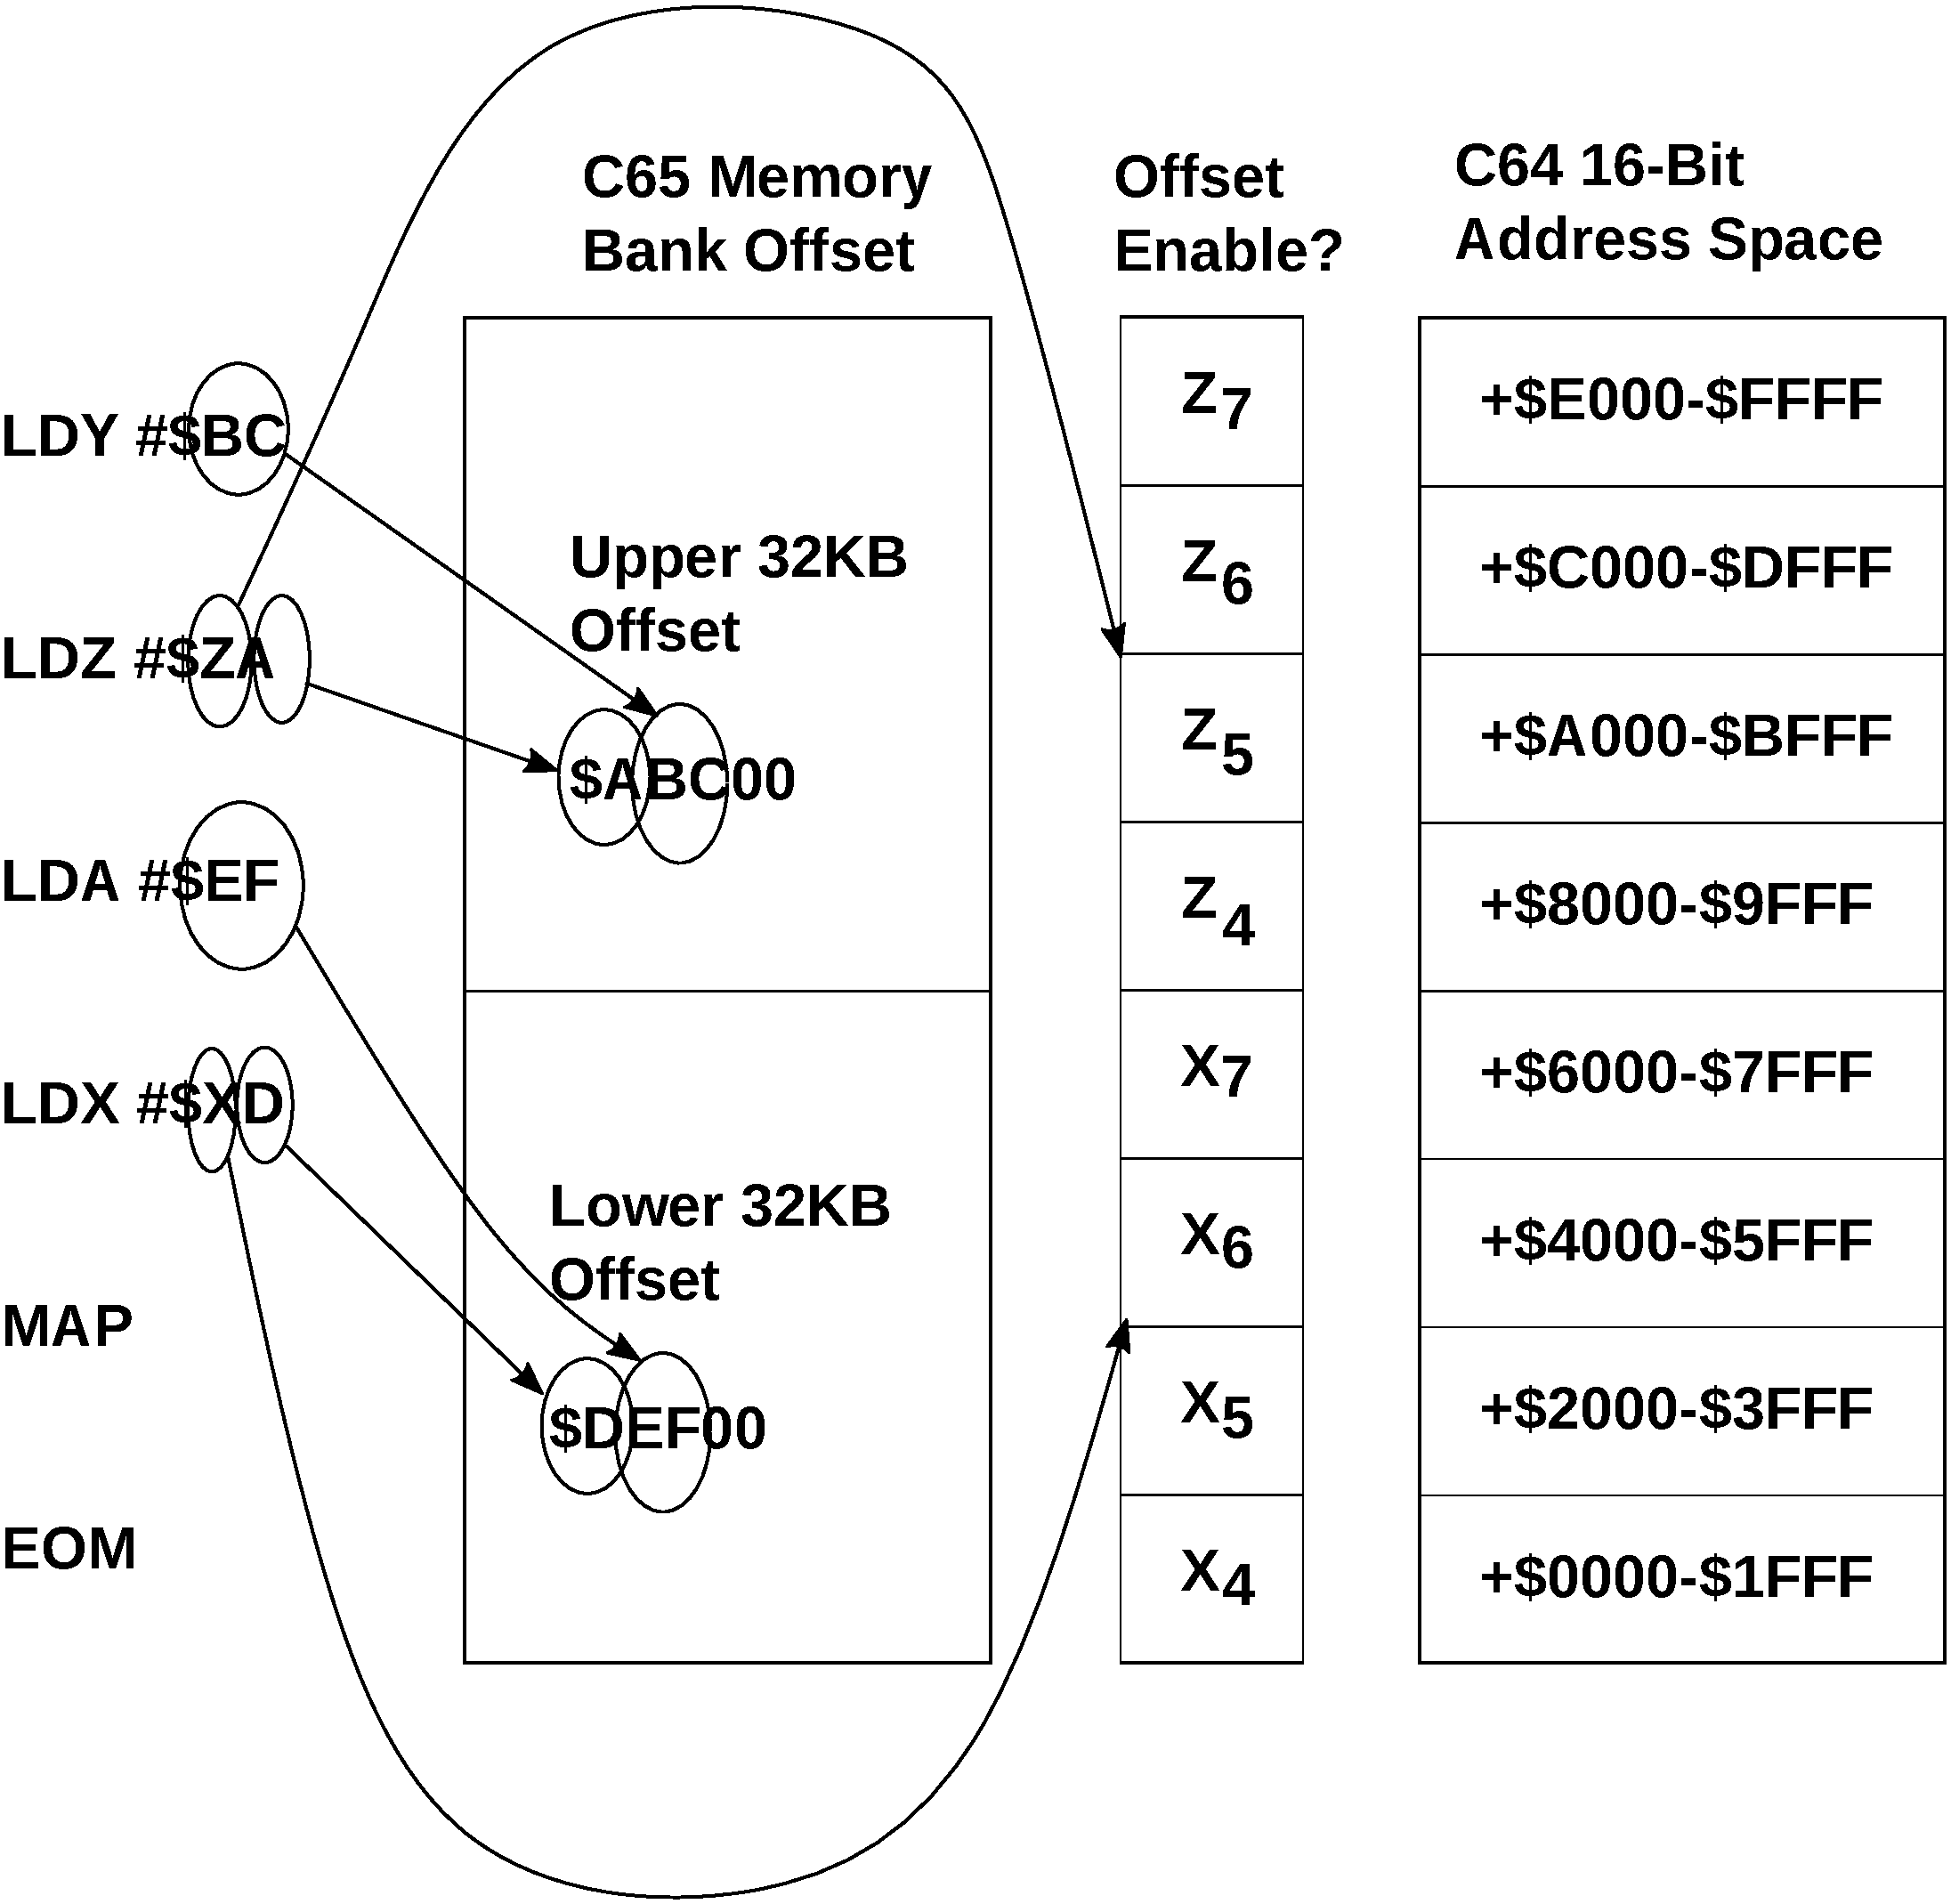
\includegraphics[width=0.75\textwidth]{images/illustrations/map-instruction-operation.pdf}\index{MAP}\index{Memory banking}
\end{center}

That is, the contents of the A register and the lower-nibble of the X register form a 12-bit value
that is multiplied by 256 to produce the offset used for any of the 8KB banks in the lower 32KB half of the 6502's 16-bit address
space.  The upper nibble of the X register is used as flags to indicate which of the four 8KB blocks in that 32KB half of the
6502 address space should have the offset added to their addresses to compute the actual address.

The Y and Z registers are used in a similar way to produce the offset for the upper 32KB half of the 6502 address space, and the
flags to indicate whether the offset is used for each of the four 8KB blocks in that half of the address space.

Note that the lower 8 bits of the offset cannot be set. That is, the offset will be a multiple of 256
bytes, unlike on some extended 6502 processors.  However, in practice this restriction is rarely
limiting.

To understand how this works in practice, the following example shows how this works with a concrete
example, showing the address ranges that would be visible in each of the 8KB slices of the 6502's
64KB address space:

\begin{center}
  \includegraphics[width=0.75\textwidth]{images/illustrations/map-instruction-operation-example1.pdf}\index{MAP}\index{Memory banking}
\end{center}

Notice that the offsets for each of the two 32KB address ranges get added to the 6502 address.
This is why the offset of \$48000 for the upper 32KB generates an address of \$50000 at the 6502
address \$8000.

See also under ``Using the MAP instruction to access >1MB'' for further explanation.

\subsubsection{Direct Memory Access (DMA) Controller}

The C65's F018/F018A DMA controller allows for rapid filling, copying and swapping of the contents of memory
anywhere in the 1MB address space. Detailed information about the F018 DMA controller, and the MEGA65's
enhancements to this, refer to \bookvref{cha:dmagic}

\subsubsection{Flat Memory Access}

\subsection{Accessing memory beyond the 1MB point}
\label{sec:extended-memory}

The MEGA65 can support up to 256MB of memory. This is more than the 1MB address space of the CSG4510
on which it is based. There are several ways of performing this.

\subsubsection{Using the MAP instruction to access >1MB}

The full address space is available to the MAP instruction for legacy C65-style memory
mapping, although some care is required, as the MAP instruction must be called up to three times.
The reason for this is that the MAP instruction must be called to first select which mega-byte of
memory will be used for the lower and upper map regions, before it is again called in the normal
way to set the memory mapping.  Because between these two calls the memory mapping offset will be
a mix of the old and new addresses, all mapping should be first disabled via the MAP instruction.
This means that the code to re-map memory should live in the bottom 64KB of RAM or in one of the
ROM-bankable regions, so that it can remain visible during the mapping process.

Failure to handle this situation properly will result in the processor executing instructions
from somewhere unexpected half-way through the process, because the routine it is executing
to perform the mapping will suddenly no longer be mapped.

Because of the relative complexity of this process, and the other problems with the MAP instruction
as a means of memory access, we recommend that for accessing data outside of the current memory
map that you use either DMA or the flat-memory address features of the 45GS02 that are described below.
Indeed, access to the full address space via the MAP instruction is only provided for completeness.

As an other example of how the MAP instruction can be used to map an area of memory from
the expanded address space, the following program maps the Ethernet frame buffer from its natural location
at \$FFDE8000 to appear at \$6800.  To keep the example as simple as possible, we assume that the code
is running from in the bottom 64KB of RAM, and not in the region between \$6000 -- \$8000.

As the MAP instruction normally is only aware of the C65-style 20-bit addresses, the MEGA65 extension to the
instruction must be used to set the upper 8 bits of the 28-bit MEGA65 addresses, i.e., which mega-byte of address
space should be used for the address translation.  This is done by setting the X
register to \$0F when setting the mega-byte number for the lower-32KB of the C64-style 64KB address space.
This does not create any incompatibility with any sensible use of the MAP instruction on a C65, because this
value indicates that none of the four 8KB memory blocks will be re-mapped, but at the same time specifies that
the upper 4 bits of the address offset for re-mapped block is the non-zero value of \$F.  The mega-byte number
is then specified by setting the A register.

The same approach applies to the upper 32KB, but using the Z and Y
registers instead of the X and A registers.  However, in this case, we do not need to re-map the upper 32KB of
memory in this example, we will leave the Z and Y registers set to zero.  We must however set X and A to
set the mega-byte number for the lower-32KB to \$FF. Therefore A must have the value \$FF.  To set the lower 20-bits
of the address offset we use the MAP instruction a second time, this time using it in the normal C65 manner.
As we want to remap \$6800 to \$FFDE800, and have already dealt with the \$FFxxxxx offset via the mega-byte number,
we need only to apply the offset to make \$6800 point to \$DE800. \$DE800 minus \$6800 = \$D8000.  As the MAP instruction
operates with a mapping granularity of 256 bytes = \$100, we can drop the last two digits from \$D8000 to obtain the
MAP offset of \$D80. The lower 8-bits, \$80, must be loaded into the A register. The upper 4-bits, \$D, must be loaded into
the low-nibble of the X register.  As we wish to apply the mapping to only the fourth of the 8KB blocks that make up the
lower 32KB half of the C64 memory map, we must set the 4th bit of the upper nibble. That is, the upper nibble must be set
to \%1000, i.e., \$8.  Therefore the X register must be loaded with \$8D.  Thus we yield the complete example program:

\begin{screenoutput}
; Map Ethernet registers at $6000 - $7FFF

; Ethernet controller really lives $FFDE000 - $FFDEFFF, so select $FF megabyte section for MAP LO
LDA #$ff
LDX #$0f
LDY #$00
LDZ #$00
map

; now enable mapping of $DE000-$DFFFF at $6000
; MAPs are offset based, so we need to subtract $6000 from the target address
; $DE000 - $6000 = $D8000
LDA #$80
LDX #$8d
LDY #$00
LDZ #$00
map
EOM

; Ethernet buffer now visible at $6800 - $6FFF
\end{screenoutput}

Note that the EOM (End Of Mapping) instruction (which is the same as NOP on a 6502, i.e., opcode \$EA) was only supplied after the last MAP instruction, to make sure that no interrupts could occur while
the memory map contained mixed values with the mega-byte number set, but the lower-bits of the mapping address had not been
updated.

No example in BASIC for the MAP instruction is possible, because the MAP is an machine code instruction of the 4510 / 45GS02 processors.

\subsubsection{Flat-Memory Access}

The 45GS02 makes it easy to read or write a byte from anywhere in memory by allowing the Zero-Page Indirect
addressing mode to use a 32-bit pointer instead of the normal 16-bit pointer.  This is accomplished by
using the Z-indexed Zero-Page Indirect Addressing Mode for the access, and having the instruction directly
preceded by a NOP instruction (opcode \$EA).  For example:

\begin{screenoutput}
NOP
LDA ($45),Z
\end{screenoutput}

If you are using the ACME assembler, or another assembler that supports the 45GS02 extensions, you can instead use square-brackets
to indicate that you are performing a flat-memory operation. Such assemblers will insert the \$EA prefix automatically for you. For example:

\begin{screenoutput}
LDA [$45],Z
\end{screenoutput}

Regardless which tool you are using, this example would read the four bytes of Zero-Page memory at \$45 -- \$48 to form a 32-bit memory address, and add the value of the
Z register to this to form the actual address that will be read from.  The byte order in the address is the same as
the 6502, i.e., the right-most (least significant) byte of the address will be read from the first address (\$45 in this case),
and so on, until the left-most (most significant) byte will be read from \$48.  For example, to read from memory location
\$12345678, the contents of memory beginning at \$45 should be 78 56 34 12.

This method is much more efficient and also simpler than either using the MAP instruction or the DMA controller for single memory accesses,
and is what we generally recommend.  The DMA controller can be used for moving/filler larger regions of memory.
We recommend the MAP instruction only be used for banking code, or in rare situations where extensive access to a small region of
memory is required, and the extra cycles of reading the 32-bit addresses is problematic.

\subsection{Virtual 32-bit Register}

The 45GS02 allows the use of its four general purpose registers, A, X, Y and Z (A is LSB, Z is MSB) as a single virtual 32-bit register, 
also called the {\em Q pseudo register}.
This can greatly simplify and speed up many common operations, and help avoid many common programming errors.
For example, adding two 16-bit or 32-bit values can now be easily accomplished with something like:

\begin{screenoutput}
  ; Clear carry before performing addition, as normal
  CLC
  ; Prefix an instruction with two NEG instructions to select virtual 32-bit register mode
  NEG
  NEG
  LDA $1234  ; Load the contents of $1234-$1237 into A,X,Y and Z respectively
  ; And again, for the addition
  NEG
  NEG
  ADC $1238  ; Add the contents of $1238-$123B
  ; The result of the addition is now in A, X, Y and Z.
  ; And can be written out in whole or part

  ; To write it all out, again, we need the NEG + NEG prefix
  NEG
  NEG
  STA $123C ; Write the whole out to $123C-$123F

  ; Or to write out the bottom bytes, we can just write the contents of A and X as normal
  STA $1240
  STX $1241
\end{screenoutput}

This approach works with the LDA, STA, ADC, SBC, CMP, EOR, AND, BIT, ORA, ASL, ASR, LSR, ROL, ROR, INC and DEC instructions.
If you are using ACME or another 45GS02 aware assembler, you can instead use the new \stw{LDQ}, \stw{STQ}, \stw{ADCQ},
\stw{SBCQ}, \stw{CPQ}, \stw{EORQ}, \stw{ANDQ}, \stw{BITQ}, \stw{ORQ}, \stw{ASLQ}, \stw{ASRQ}, \stw{LSRQ}, \stw{ROLQ}, \stw{RORQ}, \stw{INQ} and \stw{DEQ}
mnemonics.\index{LDQ}\index{STQ}\index{ADCQ}\index{SBCQ}\index{CPQ}\index{EORQ}\index{ANDQ}\index{BITQ}\index{ORQ}\index{ASLQ}\index{ASRQ}\index{LSRQ}\index{ROLQ}\index{RORQ}\index{INQ}\index{DEQ} The previous example would thus become:

\begin{screenoutput}
  ; Clear carry before performing addition, as normal
  CLC
  LDQ  $1234  ; Load the contents of $1234-$1237 into A,X,Y and Z respectively
  ADCQ $1238  ; Add the contents of $1238-$123B
  ; The result of the addition is now in A, X, Y and Z.
  ; And can be written out in whole or part

  ; To write it all out, again, we need the NEG + NEG prefix
  STQ $123C ; Write the whole out to $123C-$123F

  ; Or to write out the bottom bytes, we can just write the contents of A and X as normal
  STA $1240
  STX $1241
\end{screenoutput}

The virtual 32-bit addressing mode works with any addressing mode.
However, indexed addressing modes, where X, Y or Z are added to the address should
be used with care, because these registers may in fact be holding part of a 32-bit value.

The exception is the Zero-Page Indirect Z-Indexed addressing mode: In this case the Z register is NOT added to the target address
(with the exception of the LDQ opcode), unlike would normally be the case. This is to allow the virtual 32-bit register to be able
to be used with flat-memory access with the combined prefix of \stw{NEG NEG NOP},  before the instruction to allow accessing a
32-bit value anywhere in memory in a single instruction.

Note that the virtual 32-bit register cannot be used in immediate mode, e.g., to load a constant into the four general
purpose registers, or to add or subtract a constant value.  This is to avoid problems with variable length instructions.

For LDQ and STQ, it would save at most one byte
compared to LDA \#\$nn ... LDZ \#\$nn, and would be no faster.  In fact, for many common
values, such as \#\$00000000, there are short-cuts, such as:

\begin{screenoutput}
LDA #$00
TAX
TAY
TAZ
\end{screenoutput}

If you need to add or subtract a 32-bit immediate value, this may require you to re-order the arguments, or perform other
minor gymnastics.  For example, to compute the sum of the contents of memory and an immediate value, you can load the A, X, Y
and Z registers with the immediate value, and then use \stw{ADCQ} with the memory address, e.g.:

\begin{screenoutput}
  ; Get the immediate value #$12345678 into Q
  LDA #$78
  LDX #$56
  LDY #$34
  LDZ #$12
  ; Add the contents of memory locations $1234-$1237
  NEG
  NEG
  ADC $1234
  ; Store the result back in $1234-$1237
  NEG
  NEG
  STA $1234
\end{screenoutput}

Again, if you are using the ACME or another 45GS02-aware assembler, this can be more compactly and
clearly written as follows. But note that in both cases the same byte-sequence of machine code is
produced, and the program will take the same number of cycles to execute.

\begin{screenoutput}
  ; Get the immediate value #$12345678 into Q
  LDA #$78
  LDX #$56
  LDY #$34
  LDZ #$12
  ; Add the contents of memory locations $1234-$1237
  ADCQ $1234
  ; Store the result back in $1234-$1237
  STQ $1234
\end{screenoutput}

\section{C64 CPU Memory Mapped Registers}

\input{regtable_CPU.C64}

\section{New CPU Memory Mapped Registers}

\input{regtable_CPU.MEGA65}

\section{MEGA65 CPU Maths Acceleration Registers}

Every MEGA65 contains a combined 32-bit hardware multiplier and divider.
This device takes two 32-bit inputs, {\bf MULTINA} and {\bf MULTINB}, and simultaneously calculates:

\begin{itemize}
\item the 64-bit product {\bf MULTOUT} of {\bf MULTINA} and {\bf MULTINB}
\item the 32-bit whole part {\bf DIVOUT}(4-7) of {\bf MULTINA} divided by {\bf MULTINB}
\item the 32-bit fractional part {\bf DIVOUT}(0-3) of {\bf MULTINA} divided by {\bf MULTINB}
\end{itemize}

It is always updating the outputs based on the inputs, so there is no need to take special action when changing the inputs.
The multiplier takes 1 cycle to calculate, and the updated result will thus be available immediately (a {\bf MULBUSY} bit is
defined, but currently it won't be set at all). The hardware divider, however, can take upto 20 cycles depending on the
particular inputs. The programmer should check the {\bf DIVBUSY} bit if the divider is still calculating:

\begin{screenoutput}
loop:   BIT $D70F   ; transfer DIVBUSY bit into N flag
        BMI loop    ; as long as it is set, we need to wait
\end{screenoutput}

The MEGA65 is planned to also include a programmable math unit, which helps to accelerate the calculation of fixed-point formulae.
This is presently disabled and will be further documented if and when it becomes available (addresses \$D780 - \$D7E3).

\input{regtable_MATH.MEGA65}

\section{MEGA65 Hypervisor Mode}
\label{sec:hypervisor-mode}

\subsection{Reset}

On power-up or reset, the MEGA65 starts up in hypervisor mode, and expects to find a program in the
16KB hypervisor memory, and begins executing instructions at address \$8100.  Normally a JMP instruction
will be located at this address, that will jump into a reset routine. That is, the 45GS02
does not use the normal 6502 reset vector. It's function is emulated by the Hyppo hypervisor program,
which fetches the address from the 6502 reset vector in the loaded client operating system when
exiting hypervisor mode.

The hypervisor memory is automatically mapped on reset to \$8000 - \$BFFF.  This special memory is not
able to mapped or in anyway accessed, except when in hypervisor mode. It can, however, always be accessed from the serial monitor/debugger
interface via its 28-bit address, \$FFF8000 -- \$FFFBFFF.  This is to protect it from accidental or malicious access from a guest operating system.

\subsection{Entering / Exiting Hypervisor Mode}

Entering the Hypervisor occurs whenever any of the following events occurs:

\begin{itemize}
\item{\bf Power-on} When the MEGA65 is first powered on.
\item{\bf Reset} If the reset line is lowered, or a watch-dog triggered reset occurs.
\item{\bf SYSCALL register accessed} The registers \$D640 - \$D67F in the MEGA65 I/O context trigger SYSCALLs when accessed.
  This is intended to be the mechanism by which a client operating system or process requests the attention of the hypervisor or operating system.
\item{\bf Page Fault} On MEGA65s that feature virtual memory, a page fault will cause a trap to hypervisor mode.
\item{\bf Certain keyboard events} Pressing \widekey{RESTORE} for >0.5 seconds, or the \specialkey{ALT} and
\specialkey{TAB} key combination traps to the hypervisor.  Typically the first is used to launch the Freeze Menu an the second to toggle the display of debug interface.
\item{\bf Accessing virtualised I/O devices} For example, if the F011 (internal 3.5'' disk drive controller) has been virtualised, then attempting to read or write sectors using this device will cause traps to the hypervisor.
  \item{\bf Executing an instruction that would lock up the CPU} A number of undocumented opcodes on the 6502 will cause the CPU to lockup.  On the MEGA65, instead of locking up, the computer will trap to the hypervisor.  This could be used to implement alternative instruction behaviours, or simply to tell the user that something bad has happened.
  \item{\bf Certain special events} Some devices can generate hypervisor-level interrupts. These are implemented as traps to the hypervisor.
\end{itemize}

The 45GS02 handles all of these in a similar manner internally:

\begin{enumerate}
\item The SYSCALL or trap address is calculated, based on the event.
\item The contents of all CPU registers are saved into the virtualisation control registers.
\item The hypervisor mode memory layout is activated, the CPU decimal flag and special purpose registers are all set to appropriate values.  The contents of the A,X,Y and Z and most other CPU flags are preserved, so that they can be accessed from the Hypervisor's SYSCALL/trap handler routine, without having to load them, thus saving a few cycles for each call.
\item The hypervisor-mode flag is asserted, and the program counter (PC) register is set to the computed address.
\end{enumerate}

All of the above happens in one CPU cycle, i.e., in 25 nano-seconds.
Returning from a SYSCALL or trap consists simply of writing to \$D67F, which
requires 125 nano-seconds, for a total overhead of 150 nano-seconds.
This gives the MEGA65 SYSCALL performance rivalling -- even beating
-- even the fastest modern computers, where the system call latency is
typically hundreds to tens of thousands of cycles \cite{soares2010flexsc}.

\subsection{Hypervisor Memory Layout}

The hypervisor memory is 16KB in size.  The first 512 bytes are
reserved for SYSCALL and system trap entry
points, with four bytes for each.  For example, the reset entry point is
at \$8100 - \$8100 + 3 = \$8100 - \$8103.
This allows 4 bytes for an instruction, typically a JMP instruction,
followed by a NOP to pad it to 4 bytes.

The full list of SYSCALLs and traps is:

\begin{longtable}{|L{1.2cm}|L{1.1cm}|C{2cm}|L{6cm}|}
\hline
{\bf{HEX}} & {\bf{DEC}} & {\bf{Name}} & {\bf{Description}} \\
\hline
\endfirsthead
\multicolumn{3}{l@{}}{\ldots continued}\\
\hline
{\bf{HEX}} & {\bf{DEC}} & {\bf{Name}} & {\bf{Description}} \\
\hline
\endhead
\multicolumn{3}{l@{}}{continued \ldots}\\
\endfoot
\hline
\endlastfoot
\small  8000 & \small 32768 & SYSCALL00 & SYSCALL 0 entry point \\
\hline
\small  8004 & \small 32772 & SYSCALL01 & SYSCALL 1 entry point \\
\hline
\small  8008 & \small 32776 & SYSCALL02 & SYSCALL 2 entry point \\
\hline
\small  800C & \small 32780 & SYSCALL03 & SYSCALL 3 entry point \\
\hline
\small  8010 & \small 32784 & SYSCALL04 & SYSCALL 4 entry point \\
\hline
\small  8014 & \small 32788 & SYSCALL05 & SYSCALL 5 entry point \\
\hline
\small  8018 & \small 32792 & SYSCALL06 & SYSCALL 6 entry point \\
\hline
\small  801C & \small 32796 & SYSCALL07 & SYSCALL 7 entry point \\
\hline
\small  8020 & \small 32800 & SYSCALL08 & SYSCALL 8 entry point \\
\hline
\small  8024 & \small 32804 & SYSCALL09 & SYSCALL 9 entry point \\
\hline
\small  8028 & \small 32808 & SYSCALL0A & SYSCALL 10 entry point \\
\hline
\small  802C & \small 32812 & SYSCALL0B & SYSCALL 11 entry point \\
\hline
\small  8030 & \small 32816 & SYSCALL0C & SYSCALL 12 entry point \\
\hline
\small  8034 & \small 32820 & SYSCALL0D & SYSCALL 13 entry point \\
\hline
\small  8038 & \small 32824 & SYSCALL0E & SYSCALL 14 entry point \\
\hline
\small  803C & \small 32828 & SYSCALL0F & SYSCALL 15 entry point \\
\hline
\small  8040 & \small 32832 & SYSCALL10 & SYSCALL 16 entry point \\
\hline
\small  8044 & \small 32836 & SECURENTR & Enter secure container trap entry point \\
\hline
\small  8048 & \small 32840 & SECUREXIT & Leave secure container trap entry point. \\
\hline
\small  804C & \small 32844 & SYSCALL13 & SYSCALL 19 entry point \\
\hline
\small  8050 & \small 32848 & SYSCALL14 & SYSCALL 20 entry point \\
\hline
\small  8054 & \small 32852 & SYSCALL15 & SYSCALL 21 entry point \\
\hline
\small  8058 & \small 32856 & SYSCALL16 & SYSCALL 22 entry point \\
\hline
\small  805C & \small 32860 & SYSCALL17 & SYSCALL 23 entry point \\
\hline
\small  8060 & \small 32864 & SYSCALL18 & SYSCALL 24 entry point \\
\hline
\small  8064 & \small 32868 & SYSCALL19 & SYSCALL 25 entry point \\
\hline
\small  8068 & \small 32872 & SYSCALL1A & SYSCALL 26 entry point \\
\hline
\small  806C & \small 32876 & SYSCALL1B & SYSCALL 27 entry point \\
\hline
\small  8070 & \small 32880 & SYSCALL1C & SYSCALL 28 entry point \\
\hline
\small  8074 & \small 32884 & SYSCALL1D & SYSCALL 29 entry point \\
\hline
\small  8078 & \small 32888 & SYSCALL1E & SYSCALL 30 entry point \\
\hline
\small  807C & \small 32892 & SYSCALL1F & SYSCALL 31 entry point \\
\hline
\small  8080 & \small 32896 & SYSCALL20 & SYSCALL 32 entry point \\
\hline
\small  8084 & \small 32900 & SYSCALL21 & SYSCALL 33 entry point \\
\hline
\small  8088 & \small 32904 & SYSCALL22 & SYSCALL 34 entry point \\
\hline
\small  808C & \small 32908 & SYSCALL23 & SYSCALL 35 entry point \\
\hline
\small  8090 & \small 32912 & SYSCALL24 & SYSCALL 36 entry point \\
\hline
\small  8094 & \small 32916 & SYSCALL25 & SYSCALL 37 entry point \\
\hline
\small  8098 & \small 32920 & SYSCALL26 & SYSCALL 38 entry point \\
\hline
\small  809C & \small 32924 & SYSCALL27 & SYSCALL 39 entry point \\
\hline
\small  80A0 & \small 32928 & SYSCALL28 & SYSCALL 40 entry point \\
\hline
\small  80A4 & \small 32932 & SYSCALL29 & SYSCALL 41 entry point \\
\hline
\small  80A8 & \small 32936 & SYSCALL2A & SYSCALL 42 entry point \\
\hline
\small  80AC & \small 32940 & SYSCALL2B & SYSCALL 43 entry point \\
\hline
\small  80B0 & \small 32944 & SYSCALL2C & SYSCALL 44 entry point \\
\hline
\small  80B4 & \small 32948 & SYSCALL2D & SYSCALL 45 entry point \\
\hline
\small  80B8 & \small 32952 & SYSCALL2E & SYSCALL 46 entry point \\
\hline
\small  80BC & \small 32956 & SYSCALL2F & SYSCALL 47 entry point \\
\hline
\small  80C0 & \small 32960 & SYSCALL30 & SYSCALL 48 entry point \\
\hline
\small  80C4 & \small 32964 & SYSCALL31 & SYSCALL 49 entry point \\
\hline
\small  80C8 & \small 32968 & SYSCALL32 & SYSCALL 50 entry point \\
\hline
\small  80CC & \small 32972 & SYSCALL33 & SYSCALL 51 entry point \\
\hline
\small  80D0 & \small 32976 & SYSCALL34 & SYSCALL 52 entry point \\
\hline
\small  80D4 & \small 32980 & SYSCALL35 & SYSCALL 53 entry point \\
\hline
\small  80D8 & \small 32984 & SYSCALL36 & SYSCALL 54 entry point \\
\hline
\small  80DC & \small 32988 & SYSCALL37 & SYSCALL 55 entry point \\
\hline
\small  80E0 & \small 32992 & SYSCALL38 & SYSCALL 56 entry point \\
\hline
\small  80E4 & \small 32996 & SYSCALL39 & SYSCALL 57 entry point \\
\hline
\small  80E8 & \small 33000 & SYSCALL3A & SYSCALL 58 entry point \\
\hline
\small  80EC & \small 33004 & SYSCALL3B & SYSCALL 59 entry point \\
\hline
\small  80F0 & \small 33008 & SYSCALL3C & SYSCALL 60 entry point \\
\hline
\small  80F4 & \small 33012 & SYSCALL3D & SYSCALL 61 entry point \\
\hline
\small  80F8 & \small 33016 & SYSCALL3E & SYSCALL 62 entry point \\
\hline
\small  80FC & \small 33020 & SYSCALL3F & SYSCALL 63 entry point \\
\hline
\small  8100 & \small 33024 & RESET & Power-on/reset entry point \\
\hline
\small  8104 & \small 33028 & PAGFAULT & Page fault entry point (not currently used) \\
\hline
\small  8108 & \small 33032 & RESTORKEY & Restore-key long press trap entry point \\
\hline
\small  810C & \small 33036 & ALTTABKEY & ALT+TAB trap entry point \\
\hline
\small  8110 & \small 33040 & VF011RD & F011 virtualised disk read trap entry point \\
\hline
\small  8114 & \small 33044 & VF011WR & F011 virtualised disk write trap entry point \\
\hline
\small  8118 & \small 33048 & BREAKPT & CPU break-point encountered \\
\hline
\small  811C -- 81FB & \small 33048 -- 33275 & RESERVED & Reserved traps point entry \\
\hline
\small  81FC & \small 33276 & CPUKIL & KIL instruction in 6502-mode trap entry point \\
\hline
\end{longtable}

The remainder of the 16KB hypervisor memory is available for use by the programmer, but
will typically use the last 512 bytes for the stack and zero-page, giving an overall memory map as follows:

\begin{longtable}{|L{1.2cm}|L{1.1cm}|L{8cm}|}
\hline
{\bf{HEX}} & {\bf{DEC}} & {\bf{Description}} \\
\hline
\endfirsthead
\multicolumn{3}{l@{}}{\ldots continued}\\
\hline
{\bf{HEX}} & {\bf{DEC}} & {\bf{Description}} \\
\hline
\endhead
\multicolumn{3}{l@{}}{continued \ldots}\\
\endfoot
\hline
\endlastfoot
\small  8000 -- 81FF & \small 32768 -- 33279 & SYSCALL and trap entry points \\
\hline
\small  8200 -- BDFF & \small 33280 -- 48639 & Available for hypervisor or operating system program \\
\hline
\small  8E00 -- BEFF & \small 48640 -- 48895 & Processor stack for hypervisor or operating system \\
\hline
\small  8F00 -- BFFF & \small 48896 -- 49151 & Processor zero-page storage for hypervisor or operating system \\
\hline
\end{longtable}

The stack is used for holding the return address of function calls.  The zero-page storage is typically used for holding
variables and other short-term storage, as is customary on the 6502.

\subsection{Hypervisor Virtualisation Control Registers}

\input{regtable_HCPU.MEGA65}

\subsection{Programming for Hypervisor Mode}

The easiest way to write a program for Hypervisor Mode on the MEGA65 is to use KickC, which is a special version of C
made for writing programs for 6502-class processors.  The following example programs are from KickC's supplied examples.
KickC produces very efficient code, and directly supports the MEGA65's
hypervisor mode quite easily through the use of a linker definition file with the following contents:

\begin{screenoutput}
.file [name="%O.bin", type="bin", segments="XMega65Bin"]
.segmentdef XMega65Bin [segments="Syscall, Code, Data, Stack, Zeropage"]
.segmentdef Syscall [start=$8000, max=$81ff]
.segmentdef Code [start=$8200, min=$8200, max=$bdff]
.segmentdef Data [startAfter="Code", min=$8200, max=$bdff]
.segmentdef Stack [min=$be00, max=$beff, fill]
.segmentdef Zeropage [min=$bf00, max=$bfff, fill]
\end{screenoutput}

This file instructs KickC's assembler to create a 16KB file with the 512 byte SYSCALL/trap entry point region at the start,
followed by code and data areas, and then the stack and zero-page areas. It enforces the size and location of these fields, and
will give an error during compilation if anything is too big to fit.

With this file in place, you can then create a KickC source file that provides data structures for the SYSCALL/trap table, e.g.:

\begin{screenoutput}
// XMega65 KERNAL Development Template
// Each function of the KERNAL is a no-args function
// The functions are placed in the SYSCALLS table surrounded by JMP and NOP

import "string"

// Use a linker definition file (put the previous listing into that file)
#pragma link("mega65hyper.ld")

// Some definitions of addresses and special values that this program uses
const char* RASTER = 0xd012;
const char* VIC_MEMORY = 0xd018;
const char* SCREEN = 0x0400;
const char* BGCOL = 0xd021;
const char* COLS = 0xd800;
const char BLACK = 0;
const char WHITE = 1;

// Some text to display
char[] MESSAGE = "hello world!";
\end{screenoutput}

\begin{screenoutput}
void main() {
    // Initialise screen memory, and select correct font
    *VIC_MEMORY = 0x14;
    // Fill the screen with spaces
    memset(SCREEN, ' ', 40*25);
    // Set the colour of every character on the screen to white
    memset(COLS, WHITE, 40*25);
    // Print the "hello world!" message
    char* sc = SCREEN+40;  // Display it one line down on the screen
    char* msg = MESSAGE; // The massage to display
    // A simple copy routine to copy the string
    while(*msg) {
        *sc++ = *msg++;
    }
    // Loop forever showing two white lines as raster bars
    while(true) {
        if(*RASTER==54 || *RASTER==66) {
            *BGCOL = WHITE;
        } else {
            *BGCOL = BLACK;
        }
    }
}

// Here are a couple sample SYSCALL handlers that just display a character on the screen
void syscall1() {
    *(SCREEN+79) = '>';
}

void syscall2() {
    *(SCREEN+78) = '<';
}

// Now we select the SYSCALL segment to hold the SYSCALL/trap entry point table.
#pragma data_seg(Syscall)

// The structure of each entry point is JMP <handler address> + NOP.
// We have a char (xjmp) to hold the opcode for the JMP instruction,
// and then put the address of the SYSCALL/trap handler in the next
// two points as a pointer, and end with the NOP instruction opcode.
\end{screenoutput}

\begin{screenoutput}
struct SysCall {
    char xjmp;         // Holds $4C, the JMP $nnnn opcode
    void()* syscall;   // Holds handler address, will be the target of the JMP
    char xnop;         // Holds $EA, the NOP opcode
};

// To save writing 0x4C and 0xEA all the time, we define them as constants
const char JMP = 0x4c;
const char NOP = 0xea;

// Now we can have a nice table of up to 64 SYSCALL handlers expressed
// in a fairly readable and easy format.
// Each line is an instance of the struct SysCall from above, with the JMP
// opcode value, the address of the handler routine and the NOP opcode value.
export struct SysCall[] SYSCALLS = {
    { JMP, &syscall1, NOP },
    { JMP, &syscall2, NOP }
    };

// In this example we had only two SYSCALLs defined, so rather than having
// another 62 lines, we can just ask KickC to make the TRAP table begin
// at the next multiple of $100, i.e., at $8100.
export align(0x100) struct SysCall[] SYSCALL\_RESET = {
    { JMP, &main, NOP }
};
\end{screenoutput}

If you save the first listing into a file called mega65hyper.ld, and the second
into a file called mega65hyper.kc, you can then compile them using KickC with
a command like:

\begin{screenoutput}
  kickc -a mega65hyper
\end{screenoutput}

It will then produce a file called mega65hyper.bin, which you can then try out
on your MEGA65, or run in the XMega65 emulator with a command like:

\begin{screenoutput}
  xmega65 -kickup mega65hyper.bin
\end{screenoutput}

  \begingroup
\setlength{\def\arraystretch{1.1}\tabcolsep}{1pt}
% \OPC{Instruction}{Addr-Mode}{Bytes}{Cycles}
\newcommand{\OPC}[4]{\makecell{\begin{tabular}{>{\raggedright\arraybackslash}p{0.4cm}>{\raggedleft\arraybackslash}p{0.8cm}}
\fontsize{8pt}{0pt}\selectfont #3 & \fontsize{8pt}{0pt}\selectfont {\em #4} \\[-3pt]
\multicolumn{2}{c}{\fontsize{10pt}{0pt}\selectfont #1} \\[-3pt]
\multicolumn{2}{c}{\fontsize{8pt}{0pt}\selectfont #2}
\end{tabular}}}
\newcommand{\OPCQ}[4]{\makecell{\begin{tabular}{>{\raggedright\arraybackslash}p{0.4cm}>{\raggedleft\arraybackslash}p{0.8cm}}
\fontsize{8pt}{0pt}\selectfont #3 & \fontsize{8pt}{0pt}\selectfont {\em #4} \\[-3pt]
\multicolumn{2}{c}{\fontsize{10pt}{0pt}\selectfont #1} \\[-3pt]
\multicolumn{2}{c}{\fontsize{8pt}{0pt}\selectfont #2} \\[-12pt]
\fontsize{8pt}{0pt}\selectfont Q
\end{tabular}}}
% cell colours
\newcommand{\OPill}{\cellcolor[rgb]{1,.8,.8}}
\newcommand{\OPfar}{\cellcolor[rgb]{.8,1,.8}}
\newcommand{\OPquad}{\cellcolor[rgb]{.8,.8,1}}
\newcommand{\OPfarq}{\cellcolor[rgb]{.8,1,1}}
% binary logic
\newcommand{\binand}{$\mathit{AND}$}
\newcommand{\binor}{$\mathit{OR}$}
\newcommand{\binxor}{$\mathit{XOR}$}
\newcommand{\binnot}{$\mathit{NOT}$}
\newcommand{\binneg}{$\mathit{NEG}$}

\chapter{45GS02 \& 6502 Instruction Sets}

\section{Introduction}

The 45GS02 CPU is able to operate in native mode, where it
is compatible with the CSG 4510, and in 6502 compatibility mode,
where 6502 undocumented instructions, also known as illegal
instructions, are supported for compatibility.

\begin{quote}
{\bf WARNING:} This feature is incomplete and untested.  Most undocumented
6502 opcodes do not operate correctly when the 6502 personality is enabled.
\end{quote}

When in 4510 compatibility mode, the 45GS02 also supports a number
of extensions through {\em compound instructions}. These work be prefixing
the desired instruction's opcode with one or more {\em prefix bytes}, which
represent sequences of instructions that should not normally occur.  For example,
two \stw{NEG} instructions in a row acts as a prefix to tell the 45GS02 that the
following instruction will operate on 32 bits of data, instead of the usual 8 bits
of data.  This means that a 45GS02 instruction stream can be readily decoded or disassembled,
without needing to set special instruction length flags, as is the case with the 65816
family of microprocessors. The trade-off is increased execution time, as the 45GS02 must
skip over the prefix bytes.

The remainder of this chapter introduces the addressing modes, instructions, opcodes and
instruction timing data of the 45GS02, beginning with 6502 compatibility mode, before
moving on to 4510 compatibility mode, and the 45GS02 extensions.

\section{Stack Operations}

The stack is a area of memory where you can push data onto or fetch (pop) the latest piece
of data from it. Every stack operation that puts data to the stack (push) also changes the Stack
Pointer (SP) downwards (the stack starts at the top of the area and grows down), and every
stack operation that takes data from the stack (pop) will change the SP upwards.

So if you find something like
\begin{quote}
  STACK $\leftarrow$ VALUE
\end{quote}
implies that VALUE is pushed onto the STACK and SP is reduced by the number of bytes VALUE is
big. When pushing more than one byte, the MSB is pushed first followed by the LSB.

And in the opposite direction a operation like
\begin{quote}
  MEMORY $or$ REGISTER $\leftarrow$ STACK
\end{quote}
will pop data from the STACK and increment SP for each byte removed.

\section{Addressing Modes}
\label{sec:addressing-modes}

The 45GS02 supports 34 different addressing modes, which are explained below.
Many of these are very similar to one another, being variations of the normal 6502
or 65CE02 addressing modes, except that they accept either
32-bit pointers, operate on 32-bits of data, or both.

\subsection{Implied}

In this mode, there are no operands, as the precise function of the instruction is
implied by the instruction itself.  For example, the \screentext{INX} instruction increments
the X Register.

\subsection{Accumulator}

In this mode, the Accumulator is the operand. This is typically used to shift,
rotate or modify the value of the Accumulator Register in some way.  For example,
\screentext{INC A} increments the value in the Accumulator Register.

\subsection{Q Pseudo Register}

In this mode, the Q Pseudo Register is the operand. This is typically used to shift,
rotate or modify the value of the Q Pseudo Register in some way.  For example,
\screentext{ASLQ} shifts the value in the Q Pseudo Register left one bit.

Remember that the Q Pseudo Register is simply the A, X, Y and Z registers acting together
as a virtual 32-bit register, where A contains the least significant bits, and Z the
most significant bits. If you modify Q, you will modify the true registers, and similarly,
if you modify a true register, this will change the respective part of the Q register.

There are some cases where using a Q mode instruction can be
helpful for operating on the four true registers, for example, being able to quickly
load or store all four registers.

\subsection{Immediate Mode}

In this mode, the argument to the instruction is a value that is used directly.
This is indicated by proceeding the value with a \# character. Most assemblers allow
values to be entered in decimal, or in hexadecimal by preceding the value with a \$ sign,
in binary, by preceding the value with a \% sign.  For example, to set the Accumulator
Register to the value 5, you could use the following:

\begin{screencode}
LDA #5
\end{screencode}

The immediate argument is encoded as a single byte following the instruction.  For the above
case, the instruction stream would contain \$A9, the opcode for LDA immediate mode, followed
by \$05, the immediate operand.

\subsection{Immediate Word Mode}

In this mode, the argument is a 16-bit value that is used directly. There is only one instruction
which uses this addressing mode, \screentext{PHW}.  For example, to push the word \$1234
onto the stack, you could use:

\begin{screencode}
PHW #$1234
\end{screencode}

The low byte of the immediate value follows the opcode of the instruction.  The high byte of the
immediate value then follows that.  For the above example, the instruction stream would thus
be \$F4 \$34 \$12.

\subsection{Base-Page Mode}
\label{Base-Page (Zero-Page) Mode}

In this mode, the argument is an 8-bit address.  The upper 8-bits of the address are taken from
the Base-Page Register.  On 6502 processors, there is no Base-Page Register, and instead, the
upper 8-bits are always set to zero -- hence the name of this mode on the 6502: Zero-Page. On
the 45GS02, it is possible to move this ``Zero-Page'' to any page in the processor's 64KB view
of memory by setting the Base-Page Register using the \screentext{TAB} instruction. Base-Page
Mode allows faster access to a 256 region of memory, and uses less instruction bytes to do so.

The argument is encoded as a single byte that immediately follows the instruction opcode. For
example,

\begin{screencode}
LDA $12
\end{screencode}

would read the value stored in location \$12 in the Base-Page,
and put it into the Accumulator Register.  The instruction byte stream for this would be
\$85 \$12.

\subsection{Base-Page Quad Mode}
\label{Base-Page (Zero-Page) Quad Mode}

This mode is identical to Base-Page Mode, except that it reads a 32-bit word starting at the
specified address.

The argument is encoded as a single byte that immediately follows the instruction opcode. For
example,

\begin{screencode}
LDQ $12
\end{screencode}

would read the value stored in locations \$12 -- \$15 in the Base-Page,
and put them into the Q Pseudo Register.
The instruction byte stream for this would be \$42 \$42 \$85 \$12.  Note that this is the same as for
the Base-Page (Zero-Page) Mode, with the addition of the two \$42 prefix bytes.  Opcode \$42 is normally
NEG (negate the value in the A register).  When executed twice in a row, this returns the A value to its
original value.  The 45GS02 processor has special logic to recognises this sequence, so that it knows
to execute the next instruction using the Q Pseudo Register for that instruction.

See the note on page \pageref{Base-Page (Zero-Page) Mode} for more information about Base-Page and Zero-Page.

\subsection{Base-Page X-Indexed Mode}

This mode is identical to Base-Page Mode, except that the address is formed by taking the
argument, and adding the value of the X Register to it.  In 6502 mode, the result will always
be in the Base-Page, that is, any carry due to the addition from the low byte into the high byte
of the address will be ignored.  The encoding for this addressing mode is identical to Base-Page
Mode.

The argument is encoded as a single byte that immediately follows the instruction opcode.
For example,

\begin{screencode}
LDA $12,X
\end{screencode}

would read the value stored in location (\$12 + X) in the Base-Page,
and put it into the A register.  The instruction byte stream for this would be \$B5 \$12.

See the note on page \pageref{Base-Page (Zero-Page) Mode} for more information about Base-Page and Zero-Page.

\subsection{Base-Page Quad X-Indexed Mode}

This mode is identical to Base-Page Quad Mode, except that the address is formed by taking the
argument, and adding the value of the X Register to it.  In 6502 mode, the result will always
be in the Base-Page, that is, any carry due to the addition from the low byte into the high byte
of the address will be ignored.  The encoding for this addressing mode is identical to Base-Page Quad
Mode.

The argument is encoded as a single byte that immediately follows the instruction opcode.
For example,

\begin{screencode}
DEQ $12,X
\end{screencode}

would increment the 32-bit word stored at (\$12 + X) through to (\$15 + X) in the Base-Page,
and put it into the X register.  The instruction byte stream for this would be \$42 \$42 \$D6 \$12.

Note that LDQ is not available in this addressing mode.

See the note on page \pageref{Base-Page (Zero-Page) Mode} for more information about Base-Page and Zero-Page.
See the note on page \pageref{Base-Page (Zero-Page) Quad Mode} for more information on Quad Mode instructions.

\subsection{Base-Page Y-Indexed Mode}

This mode is identical to Base-Page Mode, except that the address is formed by taking the
argument, and adding the value of the Y Register to it.  In 6502 mode, the result will always
be in the Base-Page, that is, any carry due to the addition from the low byte into the high byte
of the address will be ignored.  The encoding for this addressing mode is identical to Base-Page
Mode.

The argument is encoded as a single byte that immediately follows the instruction opcode.
For example,

\begin{screencode}
LDX $12,Y
\end{screencode}

would read the value stored in location (\$12 + Y) in the Base-Page,
and put it into the X register.  The instruction byte stream for this would be \$B6 \$12.

See the note on page \pageref{Base-Page (Zero-Page) Mode} for more information about Base-Page and Zero-Page.


% Disabled: "no instructions currently offer this addressing mode"
\iffalse
\subsection{Base-Page Quad Y-Indexed Mode}

This mode is identical to Base-Page Quad Mode, except that the address is formed by taking the
argument, and adding the value of the Y Register to it.  In 6502 mode, the result will always
be in the Base-Page, that is, any carry due to the addition from the low byte into the high byte
of the address will be ignored.  The encoding for this addressing mode is identical to Base-Page Quad
Mode.

Note that no instructions currently offer this addressing mode.

See the note on page \pageref{Base-Page (Zero-Page) Mode} for more information about Base-Page and Zero-Page.
\fi

% Disabled: "no instructions currently offer this addressing mode"
\iffalse
\subsection{Base-Page Z-Indexed Mode}

This mode is identical to Base-Page Mode, except that the address is formed by taking the
argument, and adding the value of the Z Register to it.  In 6502 mode, the result will always
be in the Base-Page, that is, any carry due to the addition from the low byte into the high byte
of the address will be ignored.  The encoding for this addressing mode is identical to Base-Page
Mode.

Note that no instructions currently offer this addressing mode.

See the note on page \pageref{Base-Page (Zero-Page) Mode} for more information about Base-Page and Zero-Page.
\fi

% Disabled: "no instructions currently offer this addressing mode"
\iffalse
\subsection{Base-Page Quad Z-Indexed Mode}

This mode is identical to Base-Page Quad Mode, except that the address is formed by taking the
argument, and adding the value of the Z Register to it.  In 6502 mode, the result will always
be in the Base-Page, that is, any carry due to the addition from the low byte into the high byte
of the address will be ignored.  The encoding for this addressing mode is identical to Base-Page Quad
Mode.

Note that no instructions currently offer this addressing mode.

See the note on page \pageref{Base-Page (Zero-Page) Mode} for more information about Base-Page and Zero-Page.
\fi

\subsection{Absolute Mode}

In this mode, the argument is an 16-bit address.  The low 8-bits of the address are taken from
the byte immediately following the instruction opcode. The upper 8-bits are taken from the
byte following that.  For example, the instruction

\begin{screencode}
LDA $1234
\end{screencode}

would read the
memory location \$1234, and place the read value into the Accumulator Register.  This would
be encoded as \$AD \$34 \$12.

\subsection{Absolute Quad Mode}

In this mode, the argument is an 16-bit address.  The low 8-bits of the address are taken from
the byte immediately following the instruction opcode. The upper 8-bits are taken from the
byte following that.
For example, the instruction

\begin{screencode}
LDQ $1234
\end{screencode}

would read the
memory locations \$1234 -- \$1237, and place the read values into the Q Pseudo Register.  This would
be encoded as \$42 \$42 \$AD \$34 \$12.

See the note on page \pageref{Base-Page (Zero-Page) Quad Mode} for more information on Quad Mode instructions.

\subsection{Absolute X-Indexed Mode}

This mode is identical to Absolute Mode, except that the address is formed by taking the
argument, and adding the value of the X Register to it.  If the indexing causes the address
to cross a page boundary, i.e., if the upper byte of the address changes, this may incur a
1 cycle penalty, depending on the processor mode and speed setting.
The encoding for this addressing mode is identical to Absolute Mode.
For example, the instruction

\begin{screencode}
LDA $1234,X
\end{screencode}

would read the
memory location (\$1234 + X), and place the value read from there into the A Register.  This would
be encoded as \$BD \$34 \$12.

\subsection{Absolute Quad X-Indexed Mode}

This mode is identical to Absolute Quad Mode, except that the address is formed by taking the
argument, and adding the value of the X Register to it.  If the indexing causes the address
to cross a page boundary, i.e., if the upper byte of the address changes, this may incur a
1 cycle penalty, depending on the processor mode and speed setting.
The encoding for this addressing mode is identical to Absolute Quad Mode.

For example, the instruction

\begin{screencode}
ROLQ $1234,X
\end{screencode}

would rotate left the 32-bit value
at memory locations (\$1234+X) -- (\$1237+X), and write the result back to these same memory locations.  This would
be encoded as \$42 \$42 \$3E \$34 \$12.

See the note on page \pageref{Base-Page (Zero-Page) Quad Mode} for more information on Quad Mode instructions.

\subsection{Absolute Y-Indexed Mode}

This mode is identical to Absolute Mode, except that the address is formed by taking the
argument, and adding the value of the Y Register to it.  If the indexing causes the address
to cross a page boundary, i.e., if the upper byte of the address changes, this may incur a
1 cycle penalty, depending on the processor mode and speed setting.
The encoding for this addressing mode is identical to Absolute Mode.
For example, the instruction

\begin{screencode}
LDA $1234,Y
\end{screencode}

would read the
memory location (\$1234 + Y), and place the value read from there into the A Register.  This would
be encoded as \$B9 \$34 \$12.

% Disabled: "no instructions currently offer this addressing mode"
\iffalse
\subsection{Absolute Quad Y-Indexed Mode}

This mode is identical to Absolute Quad Mode, except that the address is formed by taking the
argument, and adding the value of the Y Register to it.  If the indexing causes the address
to cross a page boundary, i.e., if the upper byte of the address changes, this may incur a
1 cycle penalty, depending on the processor mode and speed setting.
The encoding for this addressing mode is identical to Absolute Quad Mode.

Note that no instructions currently offer this addressing mode.

See the note on page \pageref{Base-Page (Zero-Page) Quad Mode} for more information on Quad Mode instructions.
\fi

\subsection{Absolute Indirect Mode}

In this mode, the 16-bit argument is the address that points to, i.e., contains the
address of actual byte to read.  For example, if memory location \$1234 contains \$78
and memory location \$1235 contains \$56, then

\begin{screencode}
JMP ($1234)
\end{screencode}

would jump
to address \$5678.  The encoding for this addressing mode is identical to Absolute Mode,
 and thus this instruction would be encoded as \$6C \$34 \$12.

\subsection{Absolute Indirect X-Indexed Mode}

In this mode, the 16-bit argument is the address that points to, i.e., contains the
address of actual byte to read. It is identical to Absolute Indirect Mode, except that
 the value of the X Register is added to the pointer address.
For example, if the X Register contains the value \$04, memory location \$1238 contains \$78
and memory location \$1239 contains \$56, then

\begin{screencode}
JMP ($1234,X)
\end{screencode}

would jump
to address \$5678.
The encoding for this addressing mode is identical to Absolute Mode, and thus this instruction
would be encoded as \$7C \$34 \$12.

\subsection{Base-Page Indirect X-Indexed Mode}

This addressing mode is identical to Absolute Indirect X-Indexed Mode, except that the address
of the pointer is formed from the Base-Page Register (high byte) and the 8-bit operand (low byte).
The encoding for this addressing mode is identical to Base-Page Mode.

For example, if the X Register contains the value \$04, and the memory locations \$16 and \$17 in the current
Base-Page contained \$34 and \$12, respectively,
then

\begin{screencode}
LDA ($12,X)
\end{screencode}

would read the contents of memory location \$1234,
and store the result in the A register. This instruction would be encoded as \$A1 \$12.

See the note on page \pageref{Base-Page (Zero-Page) Mode} for more information about Base-Page and Zero-Page.

% Disabled: "no instructions currently offer this addressing mode"
\iffalse
\subsection{Base-Page Quad Indirect X-Indexed Mode}

This addressing mode is identical to Base-Page Indirect X-Indexed Mode, except that the address
of the pointer is formed from the Base-Page Register (high byte) and the 8-bit operand (low byte).
The encoding for this addressing mode is identical to Base-Page Quad Mode.

Note that no instructions currently offer this addressing mode.

See the note on page \pageref{Base-Page (Zero-Page) Mode} for more information about Base-Page and Zero-Page.
See the note on page \pageref{Base-Page (Zero-Page) Quad Mode} for more information on Quad Mode instructions.
\fi

\subsection{Base-Page Indirect Y-Indexed Mode}

This addressing mode differs from the X-Indexed Indirect modes, in that the Y Register is
added to the address that is read from the pointer, instead of being added to the pointer.
This is a very useful mode, that is frequently used because it effectively provides access to
``the Y-th byte of the memory at the address pointed to by the operand.'' That is, it de-references
a pointer.
The encoding for this addressing mode is identical to Base-Page Mode.

For example, if the Y Register contains the value \$04, and the memory locations \$12 and \$13 in the current
Base-Page contained \$78 and \$56, respectively,
then

\begin{screencode}
LDA ($12),Y
\end{screencode}

would read the contents of memory location \$567C (i.e., \$5678 + Y),
and store the result in the A register. This instruction would be encoded as \$B1 \$12.

See the note on page \pageref{Base-Page (Zero-Page) Mode} for more information about Base-Page and Zero-Page.

% Disabled: "no instructions currently offer this addressing mode"
\iffalse
\subsection{Base-Page Quad Indirect Y-Indexed Mode}

This addressing mode is identical to the Base-Page Indirect Y-Indexed Mode, except that
32-bits of data are operated on. The encoding for this addressing mode is identical to
Base-Page Mode, except that it is prefixed by \$42, \$42.

Note that no instructions currently offer this addressing mode.

See the note on page \pageref{Base-Page (Zero-Page) Mode} for more information about Base-Page and Zero-Page.
See the note on page \pageref{Base-Page (Zero-Page) Quad Mode} for more information on Quad Mode instructions.
\fi

\subsection{Base-Page Indirect Z-Indexed Mode}

This addressing mode differs from the X-Indexed Indirect modes, in that the Z Register is
added to the address that is read from the pointer, instead of being added to the pointer.
This is a very useful mode, that is frequently used because it effectively provides access to
``the Z-th byte of the memory at the address pointed to by the operand.'' That is, it de-references
a pointer.
The encoding for this addressing mode is identical to Base-Page Mode.

For example, if the Z Register contains the value \$04, and the memory locations \$12 and \$13 in the current
Base-Page contained \$78 and \$56, respectively,
then

\begin{screencode}
LDA ($12),Z
\end{screencode}

would read the contents of memory location \$567C (i.e., \$5678 + Z),
and store the result in the A register. This instruction would be encoded as \$B2 \$12.

That is, it is equivalent to the Base-Page Indirect Y-Indexed Mode, but using the Z register instead
of the Y register to calculate the offset.

See the note on page \pageref{Base-Page (Zero-Page) Mode} for more information about Base-Page and Zero-Page.

\subsection{Base-Page Quad Indirect Z-Indexed Mode}

This addressing mode is identical to the Base-Page Indirect Z-Indexed Mode, except that
32-bits of data are operated on. The encoding for this addressing mode is identical to
Base-Page Mode, except that it is prefixed by \$42, \$42.
For example, if the Z Register contains the value \$04, and the memory locations \$12 and \$13 in the current
Base-Page contained \$CD and \$AB, respectively,
then

\begin{screencode}
LDQ ($12),Z
\end{screencode}

would read the contents of memory location \$ABD1 (i.e., \$ABCD + Y) -- \$ABD4
and store the result in the Q Pseudo Register. This instruction would be encoded as \$42 \$42 \$B2 \$12.

Currently the only instruction that offers this mode is LDQ.

See the note on page \pageref{Base-Page (Zero-Page) Mode} for more information about Base-Page and Zero-Page.
See the note on page \pageref{Base-Page (Zero-Page) Quad Mode} for more information on Quad Mode instructions.

\subsection{32-bit Base-Page Indirect Z-Indexed Mode}
\label{32-bit Base-Page (Zero-Page) Indirect Z-Indexed Mode}

This mode is formed by preceding a Base-Page Indirect Z-Indexed Mode instruction with
the {NOP} instruction (opcode \$EA).  This causes the 45GS02 to read a 32-bit address instead
of a 16-bit address from the Base-Page address indicated by its operand.  The Z index is added
to that pointer.  Importantly, the 32-bit address does not refer to the processor's current 64KB
view of memory, but rather to the 45GS02's true 28-bit address space. This allows easy access
to any memory, without requiring the use of complex bank-switching or DMA operations.

For example, if addresses \$12 to \$15 contained the bytes \$20, \$30, \$FD, \$0F, representing the 32-bit address \$FFD3020, i.e., the VIC-IV border colour register's natural address, and the
Z index contained the value \$01, the following instruction sequence would change the screen
colour to blue, because the screen colour register is at \$FFD3021, i.e., \$FFD3020 + Z:

\begin{screencode}
LDA #$06
LDZ #$01
STA [$12],Z
\end{screencode}

See the note on page \pageref{Base-Page (Zero-Page) Mode} for more information about Base-Page and Zero-Page.


\subsection{32-bit Base-Page (Zero-Page) Indirect Quad Z-Indexed Mode}

This addressing mode is identical to the 32-bit Base-Page Indirect Z-Indexed Mode,
except that it operates on 32-bits of data at the 32-bit address formed by the argument,
in comparison to 32-bit Base-Page Indirect Z-Indexed Mode which operates on only 8 bits
of data.   The encoding of this addressing mode is \$42, \$42, \$EA, followed by the
natural 6502 opcode for the instruction being performed.

It is also important to note that most of the time Z is actually {\em not} added to the
pointer, as it is part of the Q Pseudo Register. Only \screentext{LDQ (\$nn),Z} will add Z.
For example,

\begin{screencode}
LDQ [$12],Z
\end{screencode}

would read the memory locations at \$12 through \$15 from the Base-Page, and use those
values to form the 32-bit address from which to load the Q Pseudo Register. The Z index is added to the 32-bit address. This instruction would be
encoded as \$42 \$42 \$EA \$B2 \$12.

See the note on page \pageref{Base-Page (Zero-Page) Mode} for more information about Base-Page and Zero-Page.
See the note on page \pageref{Base-Page (Zero-Page) Quad Mode} for more information on Quad Mode instructions.
See the note on page \pageref{32-bit Base-Page (Zero-Page) Indirect Z-Indexed Mode} for more information on 32-bit Base-Page Indirect addressing.

\subsection{Stack Relative Indirect, Y-Indexed}

This addressing mode is similar to Base-Page Indirect Y-Indexed Mode,
except that instead of providing the address of the pointer in the
Base-Page, the operand indicates the offset in the stack to find the
pointer. This addressing mode effectively de-references a pointer that
has been placed on the stack, e.g., as part of a function call from a
high-level language.  It is encoded identically to the Base-Page Mode.

For example,

\begin{screencode}
LDA ($12,SP),Y
\end{screencode}

This would use the contents of memory at the current stack pointer plus \$12 to compute the address of the pointer.
This pointer would then have the Y-Register value added to it to obtain the final address to read from, and to
store the value into the Accumulator. The instruction byte stream for this instruction would be \$E2 \$12.

If the Stack Pointer currently pointed to \$01E0, then the pointer address would
be read from addresses \$1F2 and \$1F3, i.e., the two bytes at \$1E0 + \$12 and \$1E0 + \$13.  If locations
\$1F2 and \$1F3 contained \$78 and \$56 respectively, and the Y-Register contained the value \$34, then
the final memory location that would be read would be \$5678 + \$34 = \$56AC, and the contents of that memory
location would be read into the Accumulator.

\subsection{Relative Addressing Mode}

In this addressing mode, the operand is an 8-bit signed offset to the
current value of the Program Counter (PC). It is used to allow branches
to encode the nearby address at which execution should proceed if the
branch is taken.

For example,

\begin{screencode}
BNE $2003
\end{screencode}

would jump to \$2003, if the Z flag of the processor was not set.  If this instruction were located at
address \$2000, it would be encoded as \$D0 \$01, i.e., branching to +1 bytes after the PC.  Branch
offsets greater than \$7F branch backwards, with \$FD branching to the byte immediately preceding the branch
instruction, and lower values branching progressively further back.  In this way, a branch can effectively
be made between -125 and +127 bytes from the opcode byte of the branch instruction.  For longer branches,
the 45GS02 supports Relative Word Addressing Mode, where the offset is encoded using 2 bytes instead of 1.

\subsection{Relative Word Addressing Mode}

This addressing mode is identical to Relative Addressing Mode, except that
the address offset is a 16-bit value. This allows a relative branch or jump
to any location in the current 64KB memory view.  This makes it possible
to write software that is fully relocatable, by avoiding the need for absolute
addresses when calling routines.

For example,

\begin{screencode}
BNE $3000
\end{screencode}

would jump to \$3000 if the Z flag of the process was not set. If this instruction were located at
address \$2002, it would be encoded as \$D3 \$FC \$0F, i.e., branching to +\$FFC = 4,092 bytes following
the second byte of the instruction.  The fact that the instruction is 3 bytes long is ignored in this calculation.

\clearpage
\section{6502 Instruction Set}

NOTE: The mechanisms for switching from 4510 to 6502 CPU personality
have yet to be finalised.

\subsection{Official And Unintended Instructions}

The 6502 opcode matrix has a size of 16 x 16 = 256 possible opcodes.
Those, that are officially documented, form the set of the
\textcolor{blue}{legal} instructions.
All instructions of this legal set are headed by a blue coloured mnemonic.

The remaining opcodes form the set of the
\textcolor{red}{unintended} instructions
(sometimes called "illegal" instructions).
For the sake of completeness these are documented too.
All instructions of the unintended set are headed by a red coloured mnemonic.

NOTE: The unintended instructions are currently unimplemented, and are guaranteed
not to produce exactly the same results as on other
CPU's of the 65xx family. Many of these instructions are known to
be unstable, even running on old hardware.

\subsection{Opcode Table}

The Opcode Table lists all possible opcodes, their size, cycles and addressing mode
in a conscise format.

A cell with a light red background signifies an \textcolor{red}{unintended} instruction.

\begin{center}
\begin{tabular}{c|c|c|}
  \cline{2-3}
  & \$x0 & \$x1 \\\hline
  \multicolumn{1}{|c|}{\$0x} & \OPC{OPC}{mode}{size}{cyc} & \OPill\OPC{OPC}{mode}{size}{cyc} \\\hline
\end{tabular}
\end{center}

The letters attached to the cycle count have the following meaning:

\begin{center}
  \begin{tabular}{|p{2em}|l|}
  \cline{1-2}
  & {\bf Meaning} \\\hline
\multicolumn{1}{|c|}{$b$} & Add one cycle if branch is taken. \\
                          & Add one more cycle if branch taken crosses a page boundary. \\\hline
\multicolumn{1}{|c|}{$p$} & Add one cycle if indexing crosses a page boundary. \\\hline
  \end{tabular}
\end{center}

\input{opcodetable-6502}

\addtocontents{toc}{\protect\setcounter{tocdepth}{1}}
\input{instructionset-6502}
\addtocontents{toc}{\protect\setcounter{tocdepth}{5}}

\clearpage
\section{4510 Instruction Set}

\subsection{Instruction Timing}

Note that the number of cycles depends on the speed setting of the
processor: Some instructions take more or fewer cycles when the
processor is running at full-speed, or a C65 compatibility 3.5MHz speed,
or at C64 compatibility 1MHz/2MHz speed.  More detailed information on
this is listed under each each instruction's information, but the high-level
view is:

\begin{itemize}
\item When the processor is running at 1MHz, all instructions take at least
  two cycles, and dummy cycles are re-inserted into Read-Modify-Write instructions,
  so that all instructions take exactly the same number of cycles as on a 6502.
\item The Read-Modify-Write instructions and all instructions that read a value from
  memory all require an extra cycle when operating at full speed, to allow signals
  to propagate within the processor.
\item The Read-Modify-Write instructions require an additional cycle if the operand
  is \$D019, as the dummy write is performed in this case.
  This is to improve compatibility with C64 software that frequently uses this
  ``bug'' of the 6502 to more rapidly acknowledge VIC-II interrupts.
\item Page-crossing and branch-taking penalties do not apply when the processor is
  running at full speed.
\item Many instructions require fewer cycles when the processor is running at full
  speed, as generally most non-bus cycles are removed. For example, Pushing and Pulling
  values to and from the stack requires only 2 cycles, instead of the 4 that that the
  6502 requires for these instructions.
\end{itemize}

\subsection{Opcode Table}

The coloured cells indicate an extended 45GS02 Opcode. A Q pseudo register opcode is
marked blue, a base-page indirect Z indexed opcode that can use 32-bit pointers is cyan.

\begin{center}
  \begin{tabular}{c|c|c|c|}
    \cline{2-4}
    & \$x0 & \$x1 & \$x2 \\\hline
    \multicolumn{1}{|c|}{\$0x} & \OPC{OPC}{mode}{size}{cyc} & \OPquad\OPCQ{QOP}{mode}{size}{cyc} & \OPfarq\OPCQ{FARQ}{IbpZ}{size}{cyc} \\\hline
  \end{tabular}
\end{center}

The letters attached to the cycle count have the following meaning:

\begin{center}
  \begin{tabular}{|p{2em}|l|}
  \cline{1-2}
    & {\bf Meaning} \\\hline
\multicolumn{1}{|c|}{b} & Add one cycle if branch is taken. \\
    & Add one more cycle if branch taken crosses a page boundary. \\\hline
\multicolumn{1}{|c|}{d} & Subtract one cycle when CPU is at 3.5MHz.  \\\hline
\multicolumn{1}{|c|}{i} & Add one cycle if clock speed is at 40 MHz. \\\hline
\multicolumn{1}{|c|}{m} & Subtract non-bus cycles when at 40MHz.  \\\hline
\multicolumn{1}{|c|}{p} & Add one cycle if indexing crosses a page boundary. \\\hline
\multicolumn{1}{|c|}{r} & Add one cycle if clock speed is at 40 MHz. \\\hline
\multicolumn{1}{|c|}{s} & Instruction requires 2 cycles when CPU is run at 1MHz or 2MHz. \\\hline
  \end{tabular}
\end{center}

\input{opcodetable-4510}

\addtocontents{toc}{\protect\setcounter{tocdepth}{1}}
\input{instructionset-4510}
\addtocontents{toc}{\protect\setcounter{tocdepth}{5}}

\section{45GS02 Compound Instructions}

As the 4510 has no unallocated opcodes, the 45GS02 uses compound instructions
to implement its extension.  These compound instructions consist of one or
more single byte instructions placed immediately before a conventional
instruction.  These prefixes instruct the 45GS02 to treat the following instruction
differently, as described in \bookvref{cha:cpu}.

You can find them highlighted in the 4510 Opcode Table (see \bookvref{sec:opctable4510})

% Opcodes can have multiple meanings, so no table

% No instruction timing table for compounds, as it can't
% be correctly drawn.

% Same goes for mode list.

\addtocontents{toc}{\protect\setcounter{tocdepth}{1}}
\input{instructionset-45GS02}
\addtocontents{toc}{\protect\setcounter{tocdepth}{5}}

\endgroup

  \input{appendix-reference-tables}
  \chapter{Supporters \& Donors}


The MEGA65 would not have been possible to create without the generous support of many organisations and individuals.

We are still compiling these lists, so apologies if we haven't included you yet. If you know anyone we have left out, please let us know, so that we can recognise the contribution of everyone who has made the MEGA65 possible, and into the great retro-computing project that it has become.

\section{Organisations}

{\bf The MEGA Museum of Electronic Games \& Art e.V. Germany} \\
\megakey{Everything}

{\bf Trenz Electronic, Germany} \\
\megakey{Motherboard}
\megakey{Manufacturing}
\megakey{Sales}

{\bf Hintsteiner, Austria} \\
\megakey{Case}

{\bf GMK, Germany} \\
\megakey{Keyboard}

{\bf KEVAG Telekom, Germany} \\
\megakey{Web Hosting}

\newpage
\section{Contributors}

\begin{mega65thanks}

\begin{minipage}{\linewidth}
  {\large\bf Andreas Liebeskind} \\
  \textit{(libi in paradize)} \\
  CFO MEGA eV
\end{minipage}

\begin{minipage}{\linewidth}
  {\large\bf Thomas Hertzler} \\
  \textit{(grumpyninja)} \\
  USA spokesman
\end{minipage}

\begin{minipage}{\linewidth}
  {\large\bf Russell Peake} \\
  \textit{(rdpeake)} \\
  Bug herding
\end{minipage}

\begin{minipage}{\linewidth}
  {\large\bf Alexander Nik Petra} \\
  \textit{(n0d)} \\
  Early case design
\end{minipage}

\begin{minipage}{\linewidth}
  {\large\bf Ralph Egas} \\
  \textit{(0-limits)} \\
  Business advisor
\end{minipage}

\begin{minipage}{\linewidth}
  {\large\bf Lucas Moss} \\
  MEGAphone PCB design
\end{minipage}

\begin{minipage}{\linewidth}
  {\large\bf Daren Klamer} \\
  \textit{(Impakt)} \\
  Manual proof-reading
\end{minipage}

\begin{minipage}{\linewidth}
  {\large\bf Daniël Mantione}  \\
  \textit{(dmantione)} \\
  C64 hardware guru
\end{minipage}

\columnbreak

\begin{minipage}{\linewidth}
  {\large\bf Dr. Canan Hastik} \\
  \textit{(indica)} \\
  Chairwoman MEGA eV
\end{minipage}

\begin{minipage}{\linewidth}
  {\large\bf Simon Jameson} \\
  \textit{(Shallan)} \\
  Platform enhancements
\end{minipage}

\begin{minipage}{\linewidth}
  {\large\bf Stephan Kleinert} \\
  \textit{(ubik)} \\
  Destroyer of BASIC 10
\end{minipage}

\begin{minipage}{\linewidth}
  {\large\bf Wayne Johnson} \\
  \textit{(sausage)} \\
  Manual additions
\end{minipage}

\begin{minipage}{\linewidth}
  {\large\bf L. Kleiss} \\
  \textit{(LAK132)} \\
  MegaWAT presentation software
\end{minipage}

\begin{minipage}{\linewidth}
  {\large\bf Maurice van Gils }  \\
  \textit{(Maurice)}  \\
  BASIC 65 example programs
\end{minipage}

\begin{minipage}{\linewidth}
  {\large\bf Andrew Owen}  \\
  \textit{(Cheveron)} \\
  Keyboard, Sinclair support
\end{minipage}

\begin{minipage}{\linewidth}
  {\large\bf Adam Barnes}  \\
  \textit{(amb5l)} \\
  HDMI expert and board revision
\end{minipage}

\begin{minipage}{\linewidth}
  {\large\bf Wayne Rittimann, Jr.} \\
  \textit{(johnwayner)} \\
  Bug squashing on all levels
\end{minipage}

\end{mega65thanks}


\newpage
\section{Supporters}

\begin{small}
% page 1
\setlength{\tabcolsep}{1mm}
\begin{tabular}{p{4cm}p{4cm}p{4cm}}
3c74ce64 & Arne Neumann & Christian Gräfe \\
8-Bit Classics & Arne Richard Tyarks & Christian Heffner \\
@11110110100 & Axel Klahr & Christian Kersting \\
Aaron Smith & Balaz Ondrej & Christian Schiller \\
Achim Mrotzek & Barry Thompson & Christian Streck \\
Adolf Nefischer & Bartol Filipovic & Christian Weyer \\
Adrian Esdaile & Benjamin Maas & Christian Wyk \\
Adrien Guichard & Bernard Alaiz & Christoph Haug \\
Ahmed Kablaoui & Bernhard Zorn & Christoph Huck \\
Alan Bastian Witkowski & Bieno Marti-Braitmaier & Christoph Pross \\
Alan Field & Bigby & Christopher Christopher \\
Alastair Paulin-Campbell & Bill LaGrue & Christopher Kalk \\
Alberto Mercuri & Bjoerg Stojalowski & Christopher Kohlert \\
Alexander Haering & Björn Johannesson & Christopher Nelson \\
Alexander Kaufmann & Bjørn Melbøe & Christopher Taylor \\
Alexander Niedermeier & Bo Goeran Kvamme & Christopher Whillock \\
Alexander Soppart & Boerge Noest & Claudio Piccinini \\
Alfonso Ardire & Bolko Beutner & Claus Skrepek \\
Amiga On The Lake & Brett Hallen & Collen Blijenberg \\
André Kudra & Brian Gajewski & Constantine Lignos \\
André Simeit & Brian Green & Crnjaninja \\
André Wösten & Brian Juul Nielsen & Daniel Auger \\
Andrea Farolfi & Brian Reiter & Daniel Julien \\
Andrea Minutello & Bryan Pope & Daniel Lobitz \\
Andreas Behr & Burkhard Franke & Daniel O'Connor \\
Andreas Freier & Byron Goodman & Daniel Teicher \\
Andreas Grabski & Cameron Roberton (KONG) & Daniel Tootill \\
Andreas Millinger & Carl Angervall & Daniel Wedin \\
Andreas Nopper & Carl Danowski & Daniele Benetti \\
Andreas Ochs & Carl Stock & Daniele Gaetano Capursi \\
Andreas Wendel Manufaktur & Carl Wall & Dariusz Szczesniak \\
Andreas Zschunke & Carlo Pastore & Darrell Westbury \\
Andrew Bingham & Carlos Silva & David Asenjo Raposo \\
Andrew Dixon & Carsten Sørensen & David Dillard \\
Andrew Mondt & Cenk Miroglu Miroglu & David Gorgon \\
Andrzej Hłuchyj & Chang sik Park & David Norwood \\
Andrzej Sawiniec & Charles A. Hutchins Jr. & David Raulo \\
Andrzej Śliwa & Chris Guthrey & David Ross \\
Anthony W. Leal & Chris Hooper & de voughn accooe \\
Arkadiusz Bronowicki & Chris Stringer & Dean Scully \\
Arkadiusz Kwasny & Christian Boettcher & Dennis Jeschke \\
Arnaud Léandre & Christian Eick & Dennis Schaffers \\
Arne Drews & Christian Gleinser & Dennis Schierholz \\
\end{tabular}
% page 2
\newpage
\setlength{\tabcolsep}{1mm}
\begin{tabular}{p{4cm}p{4cm}p{4cm}}
Dennis Schneck & Frank Haaland & Helge Förster \\
denti & Frank Hempel & Hendrik Fensch \\
Dick van Ginkel & Frank Koschel & Henning Harperath \\
Diego Barzon & Frank Linhares & Henri Parfait \\
Dierk Schneider & Frank Sleeuwaert & Henrik Kühn \\
Dietmar Krueger & Frank Wolf & Holger Burmester \\
Dietmar Schinnerl & FranticFreddie & Holger Sturk \\
Dirk Becker & Fredrik Ramsberg & Howard Knibbs \\
Dirk Wouters & Fridun Nazaradeh & Hubert de Hollain \\
Domingo Fivoli & Friedel Kropp & Huberto Kusters \\
DonChaos & Garrick West & Hugo Maria Gerardus v.d. Aa \\
Donn Lasher & Gary Lake-Schaal & Humberto Castaneda \\
Douglas Johnson & Gary Pearson & Ian Cross \\
Dr. Leopold Winter & Gavin Jones & IDE64 Staff \\
Dusan Sobotka & Geir Sigmund Straume & Igor Ianov \\
Earl Woodman & Gerd Mitlaender & Igor Kurtes \\
Ed Reilly & Giampietro Albiero & Immo Beutler \\
Edoardo Auteri & Giancarlo Valente & Ingo Katte \\
Eduardo Gallardo & Gianluca Girelli & Ingo Keck \\
Eduardo Luis Arana & Giovanni Medina & Insanely Interested Publishing \\
Eirik Juliussen Olsen & Glen Fraser & IT-Dienstleistungen Obsieger \\
Emilio Monelli & Glen R Perye III & Ivan Elwood \\
EP Technical Services & Glenn Main & Jaap HUIJSMAN \\
Epic Sound & Gordon Rimac & Jace Courville \\
Erasmus Kuhlmann & GRANT BYERS & Jack Wattenhofer \\
ergoGnomik & Grant Louth & Jakob Schönpflug \\
Eric Hilaire & Gregor Bubek & Jakub Tyszko \\
Eric Hildebrandt & Gregor Gramlich & James Hart \\
Eric Hill & Guido Ling & James Marshburn \\
Eric Jutrzenka & Guido von Gösseln & James McClanahan \\
Erwin Reichel & Guillaume Serge & James Sutcliffe \\
Espen Skog & Gunnar Hemmerling & Jan Bitruff \\
Evangelos Mpouras & Günter Hummel & Jan Hildebrandt \\
Ewan Curtis & Guy Simmons & Jan Iemhoff \\
Fabio Zanicotti & Guybrush Threepwood & Jan Kösters \\
Fabrizio Di Dio & Hakan Blomqvist & Jan Peter Borsje \\
Fabrizio Lodi & Hans Pronk & Jan Schulze \\
FARA Gießen GmbH & Hans-Jörg Nett & Jan Stoltenberg-Lerche \\
FeralChild & Hans-Martin Zedlitz & Janne Tompuri \\
First Choice Auto's & Harald Dosch & Jannis Schulte \\
Florian Rienhardt & Harri Salokorpi & Jari Loukasmäki \\
Forum64. de & Harry Culpan & Jason Smith \\
Francesco Baldassarri & Harry Venema & Javier Gonzalez Gonzalez \\
Frank Fechner & Heath Gallimore & Jean-Paul Lauque \\
Frank Glaush & Heinz Roesner & Jeffrey van der Schilden \\
Frank Gulasch & Heinz Stampfli & Jens Schneider \\
\end{tabular}
% page 3
\newpage
\setlength{\tabcolsep}{1mm}
\begin{tabular}{p{4cm}p{4cm}p{4cm}}
Jens-Uwe Wessling & Kenneth Joensson & Marco Cappellari \\
Jesse DiSimone & Kevin Edwards & Marco Rivela \\
Jett Adams & Kevin Thomasson & Marco van de Water \\
Johan Arneklev & Kim Jorgensen & Marcus Gerards \\
Johan Berntsson & Kim Rene Jensen & Marcus Herbert \\
Johan Svensson & Kimmo Hamalainen & Marcus Linkert \\
Johannes Fitz & Konrad Buryło & Marek Pernicky \\
John Cook & Kosmas Einbrodt & Mario Esposito \\
John Deane & Kurt Klemm & Mario Fetka \\
John Dupuis & Lachlan Glaskin & Mario Teschke \\
John Nagi & Large bits collider & Mariusz Tymków \\
John Rorland & Lars Becker & Mark Adams \\
John Sargeant & Lars Edelmann & Mark Anderson \\
John Traeholt & Lars Slivsgaard & Mark Green \\
Jon Sandelin & Lasse Lambrecht & Mark Hucker \\
Jonas Bernemann & Lau Olivier & Mark Leitiger \\
Jonathan Prosise & Lee Chatt & Mark Spezzano \\
Joost Honig & Loan Leray & Mark Watkin \\
Jordi Pakey-Rodriguez & Lorenzo Quadri & Marko Rizvic \\
Jöre Weber & Lorenzo Travagli & Markus Bieler \\
Jörg Jungermann & Lorin Millsap & Markus Bonet \\
Jörg Schaeffer & Lothar James Foss & Markus Dauberschmidt \\
Jörg Weese & Lothar Serra Mari & Markus Fehr \\
Josef Hesse & Luca Papinutti & Markus Fuchs \\
Josef Soucek & Ludek Smetana & Markus Guenther-Hirn \\
Josef Stohwasser & Lukas Burger & Markus Liukka \\
Joseph Clifford & Lutz-Peter Buchholz & Markus Merz \\
Joseph Gerth & Luuk Spaetgens & Markus Roesgen \\
Jovan Crnjanin & Mad Web Skills & Markus Uttenweiler \\
Juan Pablo Schisano & MaDCz & Martin Bauhuber \\
Juan S. Cardona Iguina & Magnus Wiklander & Martin Benke \\
JudgeBeeb & Maik Diekmann & Martin Gendera \\
Juliussen Olsen & Malte Mundt & Martin Groß \\
Juna Luis Fernandez Garcia & Manfred Wittemann & Martin Gutenbrunner \\
Jürgen Endras & Manuel Beckmann & Martin Johansen \\
Jürgen Herm Stapelberg & Manzano Mérida & Martin Marbach \\
Jyrki Laurila & Marc "3D-vice" Schmitt & Martin Sonnleitner \\
Kai Pernau & Marc Bartel & Martin Steffen \\
Kalle Pöyhönen & Marc Jensen & Marvin Hardy \\
Karl Lamford & Marc Schmidt & Massimo Villani \\
Karl-Heinz Blum & Marc Theunissen & Mathias Dellacherie \\
Karsten Engstler & Marc Tutor & Mathieu Chouinard \\
Karsten Westebbe & Marc Wink & Matthew Adams \\
katarakt & Marcel Buchtmann & Matthew Browne \\
Keith McComb & Marcel Kante & Matthew Carnevale \\
Kenneth Dyke & Marco Beckers & Matthew Palmer \\
\end{tabular}
% page 4
\newpage
\setlength{\tabcolsep}{1mm}
\begin{tabular}{p{4cm}p{4cm}p{4cm}}
Matthew Santos & Michele Porcu & Paul Jackson \\
Matthias Barthel & Miguel Angel Rodriguez Jodar & Paul Johnson \\
Matthias Dolenc & Mikael Lund & Paul Kuhnast (mindrail) \\
Matthias Fischer & Mike Betz & Paul Massay \\
Matthias Frey & Mike Kastrantas & Paul Westlake \\
Matthias Grandis & Mike Pikowski & Paul Woegerer \\
Matthias Guth & Mikko Hämäläinen & Pauline Brasch \\
Matthias Lampe & Mikko Suontausta & Paulo Apolonia \\
Matthias Meier & Mirko Roller & Pete Collin \\
Matthias Mueller & Miroslav Karkus & Pete of Retrohax.net \\
Matthias Nofer & Morgan Antonsson & Peter Eliades \\
Matthias Schonder & Moritz & Peter Gries \\
Maurice Al-Khaliedy & Morten Nielsen & Peter Habura \\
Max Ihlenfeldt & MUBIQUO APPS,SL & Peter Herklotz \\
Meeso Kim & Myles Cameron-Smith & Peter Huyoff \\
Michael Dailly & Neil Moore & Peter Knörzer \\
Michael Dötsch & Nelson & Peter Leswell \\
Michael Dreßel & neoman & Peter Weile \\
Michael Fichtner & Nicholas Melnick & Petri Alvinen \\
Michael Fong & Nikolaj Brinch Jørgensen & Philip Marien \\
Michael Geoffrey Stone & Nils Andreas & Philip Timmermann \\
Michael Gertner & Nils Eilers & Philipp Rudin \\
Michael Grün & Nils Hammerich & Pierre Kressmann \\
Michael Habel & Nils77 & Pieter Labie \\
Michael Härtig & Norah Smith & Piotr Kmiecik \\
Michael Haynes & Norman King & Power-on.at \\
Michael J Burkett & Normen Zoch & Przemysław Safonow \\
Michael Jensen & Olaf Grunert & Que Labs \\
Michael Jurisch & Ole Eitels & R Welbourn \\
Michael Kappelgaard & Oliver Boerner & R-Flux \\
Michael Kleinschmidt & Oliver Brüggmann & Rafał Michno \\
Michael Lorenz & Oliver Graf & Rainer Kappler \\
Michael Mayerhofer & Oliver Smith & Rainer Kopp \\
Michael Nurney & Olivier Bori & Rainer Weninger \\
Michael Rasmussen & ONEPSI LLC & Ralf Griewel \\
Michael Richmond & oRdYNe & Ralf Pöscha \\
Michael Sachse & Osaühing Trioflex & Ralf Reinhardt \\
Michael Sarbak & OSHA-PROS USA & Ralf Schenden \\
Michael Schneider & Padawer & Ralf Smolarek \\
Michael Scholz & Patrick Becher & Ralf Zenker \\
Michael Timm & Patrick Bürckstümmer & Ralph Bauer \\
Michael Traynor & Patrick de Zoete & Ralph Wernecke \\
Michael Whipp & Patrick Toal & Rédl Károly \\
Michal Ursiny & Patrick Vogt & Reiner Lanowski \\
Michele Chiti & Paul Alexander Warren & Remi Veilleux \\
Michele Perini & Paul Gerhardt (KONG) & Riccardo Bianchi \\
\end{tabular}
% page 5
\newpage
\setlength{\tabcolsep}{1mm}
\begin{tabular}{p{4cm}p{4cm}p{4cm}}
Richard Englert & Sigurbjorn Larusson & Thomas Niemann \\
Richard Good & Sigurdur Finnsson & Thomas Scheelen \\
Richard Menedetter & Simon Lawrence & Thomas Schilling \\
Richard Sopuch & Simon Wolf & Thomas Tahsin-Bey \\
Rick Reynolds & spreen.digital & Thomas Walter \\
Rico Gruninger & Stefan Haberl & Thomas Wirtzmann \\
Rob Dean & Stefan Kramperth & Thorsten Knoll \\
Robert Bernardo & Stefan Richter & Thorsten Nolte \\
Robert Eaglestone & Stefan Schultze & Tim Krome \\
Robert Grasböck & Stefan Sonnek & Tim Waite \\
Robert Miles & Stefan Theil & Timo Weirich \\
Robert Schwan & Stefan Vrampe & Timothy Blanks \\
Robert Shively & Stefano Canali & Timothy Henson \\
Robert Tangmar & Stefano Mozzi & Timothy Prater \\
Robert Trangmar & Steffen Reiersen & Tobias Butter \\
Rodney Xerri & Stephan Bielmann & Tobias Heim \\
Roger Olsen & Stephen Jones & Tobias Köck \\
Roger Pugh & Stephen Kew & Tobias Lüthi \\
Roland Attila Kett & Steve Gray & Tommi Vasarainen \\
Roland Evers & Steve Kurlin & Toni Ammer \\
Roland Schatz & Steve Lemieux & Tore Olsen \\
Rolf Hass & Steven Combs & Torleif Strand \\
Ronald Cooper & Stewart Dunn & Torsten Schröder \\
Ronald Hunn & Stuart Marsh & Tuan Nguyen \\
Ronny Hamida & Sven Neumann & Uffe Jakobsen \\
Ronny Preiß & Sven Stache & Ulrich Hintermeier \\
Roy van Zundert & Sven Sternberger & Ulrich Nieland \\
Rüdiger Wohlfromm & Sven Wiegand & Ulrik Kruse \\
Ruediger Schlenter & Szabolcs Bence & Urban Lindeskog \\
Rutger WIllemsen & Tantrumedia Limited & Ursula Förstle \\
Sampo Peltonen & Techvana Operations Ltd. & Uwe Anfang \\
Sarmad Gilani & Teddy Turmeaux & Uwe Boschanski \\
SAS74 & Teemu Korvenpää & Vedran Vrbanc \\
Sascha Hesse & The Games Foundation & Verm Project \\
Scott Halman & Thierry Supplisson & Wayne Rittimann \\
Scott Hollier & Thieu-Duy Thai & Wayne Sander \\
Scott Robison & Thomas Bierschenk & Wayne Steele \\
Sebastian Baranski & Thomas Edmister & Who Knows \\
Sebastian Bölling & Thomas Frauenknecht & Winfried Falkenhahn \\
Sebastian Felzmann & Thomas Gitzen & Wolfgang Becker \\
Sebastian Lipp & Thomas Gruber & Wolfgang Stabla \\
Sebastian Rakel & Thomas Haidler & Worblehat \\
Şemseddin Moldibi & Thomas Jager & www.patop69.net \\
Seth Morabito & Thomas Karlsen & Yan B \\
Shawn McKee & Thomas Laskowski & Zoltan Markus \\
Siegfried Hartmann & Thomas Marschall & Zsolt Zsila \\
Zytex Online Store &  &  \\
\end{tabular}
\end{small}
\ifdefined\printmanual
\else
\setstretch{1}
\fi



\nocite{*}
\bibliographystyle{IEEEtran}
\bibliography{references}

\printindex

\input{common-footer}

